\section{Results}
%%%%%%%%%%%% MID WAY AGENDA %%%%%%%%%%%%%%
\begin{frame}<beamer>
\vspace*{1.5cm}
\begin{figure}
\centering
% This file was created by matlab2tikz.
%
%The latest updates can be retrieved from
%  http://www.mathworks.com/matlabcentral/fileexchange/22022-matlab2tikz-matlab2tikz
%where you can also make suggestions and rate matlab2tikz.
%
\definecolor{mycolor1}{rgb}{0.00000,0.44700,0.74100}%
\definecolor{mycolor2}{rgb}{0.85000,0.32500,0.09800}%
%
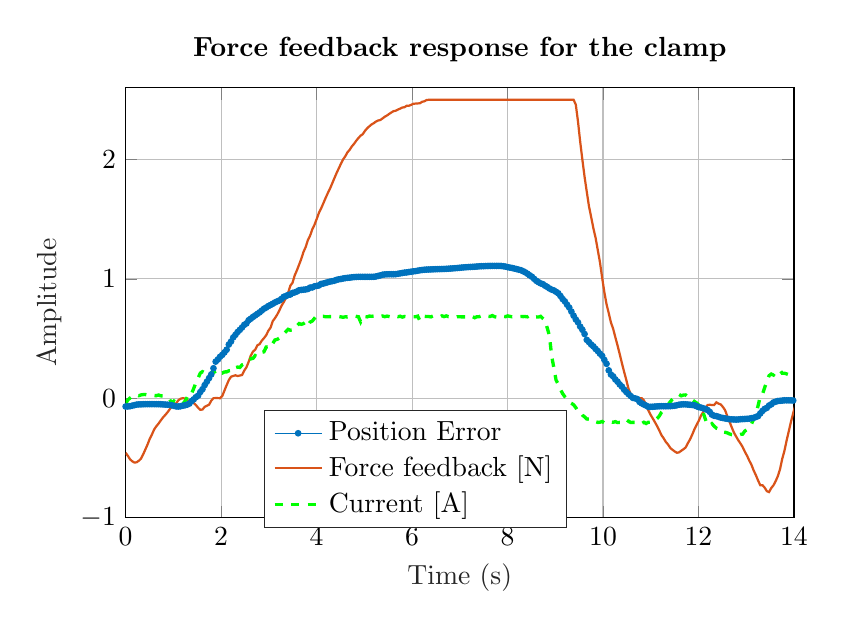
\begin{tikzpicture}

\begin{axis}[%
width=0.7\columnwidth,
height=0.45\columnwidth,
at={(2.512in,1.147in)},
scale only axis,
xmin=0,
xmax=14,
xlabel style={font=\color{white!15!black}},
xlabel={Time (s)},
ymin=-1,
ymax=2.6,
ylabel style={font=\color{white!15!black}},
ylabel={Amplitude},
axis background/.style={fill=white},
title style={font=\bfseries},
title={Force feedback response for the clamp},
xmajorgrids,
ymajorgrids,
legend style={legend cell align=left, align=left, draw=white!15!black, at={(0.66,0.25)}}
]

\addplot [color=mycolor1, draw=none, mark=*, mark size=1,mark options={solid, mycolor1}]
  table[row sep=crcr]{%
0	-0.069839\\
0.046	-0.0691929999999998\\
0.092	-0.0674169999999998\\
0.138	-0.0627580000000001\\
0.184	-0.0585599999999999\\
0.23	-0.053715\\
0.276	-0.052262\\
0.322	-0.0517779999999999\\
0.368	-0.0508089999999999\\
0.414	-0.050325\\
0.46	-0.0500019999999999\\
0.506	-0.0500019999999999\\
0.552	-0.0500019999999999\\
0.598	-0.0500019999999999\\
0.644	-0.050233\\
0.69	-0.0504629999999999\\
0.736	-0.0509360000000001\\
0.782	-0.0523979999999999\\
0.828	-0.0533170000000001\\
0.874	-0.0544640000000001\\
0.92	-0.0558380000000001\\
0.966	-0.059431\\
1.012	-0.0646089999999999\\
1.058	-0.069102\\
1.104	-0.070166\\
1.15	-0.0678619999999999\\
1.196	-0.0632820000000001\\
1.242	-0.0596559999999999\\
1.288	-0.054314\\
1.334	-0.045984\\
1.38	-0.0253700000000001\\
1.426	-0.00976399999999988\\
1.472	0.00805999999999996\\
1.518	0.0212249999999999\\
1.564	0.051482\\
1.61	0.0750869999999999\\
1.656	0.109672\\
1.702	0.138343\\
1.748	0.168177\\
1.794	0.199188\\
1.84	0.250473\\
1.886	0.306211\\
1.932	0.324103\\
1.978	0.347052\\
2.024	0.362787\\
2.07	0.383776\\
2.116	0.406007\\
2.162	0.449559\\
2.208	0.474824\\
2.254	0.508958\\
2.3	0.530804\\
2.346	0.554437\\
2.392	0.572537\\
2.438	0.591942\\
2.484	0.614258\\
2.53	0.625926\\
2.576	0.652916\\
2.622	0.665954\\
2.668	0.680707\\
2.714	0.6931054\\
2.76	0.7064931\\
2.806	0.7187228\\
2.852	0.7341136\\
2.898	0.7492224\\
2.944	0.7593239\\
2.99	0.7720971\\
3.036	0.7809118\\
3.082	0.7910974\\
3.128	0.8020223\\
3.174	0.81066\\
3.22	0.8186307\\
3.266	0.8319814\\
3.312	0.8492741\\
3.358	0.8558223\\
3.404	0.8646376\\
3.45	0.868742\\
3.496	0.8814436\\
3.542	0.8863328\\
3.588	0.8938385\\
3.634	0.9044656\\
3.68	0.9069801\\
3.726	0.9089659\\
3.772	0.9109976\\
3.818	0.9148639\\
3.864	0.9265554\\
3.91	0.9278963\\
3.956	0.9373217\\
4.002	0.940841\\
4.048	0.9445568\\
4.094	0.95726415\\
4.14	0.9604788\\
4.186	0.96597617\\
4.232	0.97119919\\
4.278	0.97641396\\
4.324	0.9801821\\
4.37	0.9838232\\
4.416	0.9907857\\
4.462	0.99572\\
4.508	0.9983443\\
4.554	1.0027004\\
4.6	1.0057562\\
4.646	1.0081051\\
4.692	1.0098843\\
4.738	1.0125273\\
4.784	1.0145615\\
4.83	1.015724\\
4.876	1.0164667\\
4.922	1.0164667\\
4.968	1.0164667\\
5.014	1.0164667\\
5.06	1.0164667\\
5.106	1.0164667\\
5.152	1.0164667\\
5.198	1.017048\\
5.244	1.0196638\\
5.29	1.0246052\\
5.336	1.0286748\\
5.382	1.0344887\\
5.428	1.0368141\\
5.474	1.0379768\\
5.52	1.0385582\\
5.566	1.0385582\\
5.612	1.0385582\\
5.658	1.0391396\\
5.704	1.0420462\\
5.75	1.045534\\
5.796	1.0490214\\
5.842	1.0522178\\
5.888	1.0536705\\
5.934	1.0571568\\
5.98	1.059633\\
6.026	1.062445\\
6.072	1.0644935\\
6.118	1.0679936\\
6.164	1.0718006\\
6.21	1.0739226\\
6.256	1.0760766\\
6.302	1.0773746\\
6.348	1.0781606\\
6.394	1.0786866\\
6.44	1.0796386\\
6.486	1.0806226\\
6.532	1.0811326\\
6.578	1.0815816\\
6.624	1.0821676\\
6.67	1.0826356\\
6.716	1.0836156\\
6.762	1.0849286\\
6.808	1.0862066\\
6.854	1.0874876\\
6.9	1.0889816\\
6.946	1.0904386\\
6.992	1.0921886\\
7.038	1.0943516\\
7.084	1.0958206\\
7.13	1.0971756\\
7.176	1.0983656\\
7.222	1.0995076\\
7.268	1.1005966\\
7.314	1.1015086\\
7.36	1.1031166\\
7.406	1.1045566\\
7.452	1.1057716\\
7.498	1.1059546\\
7.544	1.1072416\\
7.59	1.1076566\\
7.636	1.1080086\\
7.682	1.1083606\\
7.728	1.1083606\\
7.774	1.1082496\\
7.82	1.1082496\\
7.866	1.1078506\\
7.912	1.1055066\\
7.958	1.1023436\\
8.004	1.0977176\\
8.05	1.0940366\\
8.096	1.0909596\\
8.142	1.0861036\\
8.188	1.0816106\\
8.234	1.0766646\\
8.28	1.0723386\\
8.326	1.0637863\\
8.372	1.0543818\\
8.418	1.0428257\\
8.464	1.029448\\
8.51	1.0175659\\
8.556	1.0002029\\
8.602	0.9837055\\
8.648	0.97187785\\
8.694	0.96156563\\
8.74	0.9554396\\
8.786	0.942303\\
8.832	0.9318928\\
8.878	0.9191614\\
8.924	0.9095359\\
8.97	0.9029574\\
9.016	0.8912888\\
9.062	0.879097\\
9.108	0.8563865\\
9.154	0.8307516\\
9.2	0.8113894\\
9.246	0.7837317\\
9.292	0.7592755\\
9.338	0.725409\\
9.384	0.691096\\
9.43	0.659743\\
9.476	0.635184\\
9.522	0.599631\\
9.568	0.572746\\
9.614	0.537474\\
9.66	0.488529\\
9.706	0.470013\\
9.752	0.449131\\
9.798	0.434072\\
9.844	0.412879\\
9.89	0.394881\\
9.936	0.372667\\
9.982	0.354272\\
10.028	0.320757\\
10.074	0.287993\\
10.12	0.232964\\
10.166	0.197741\\
10.212	0.18275\\
10.258	0.156795\\
10.304	0.138484\\
10.35	0.114872\\
10.396	0.097008\\
10.442	0.071595\\
10.488	0.05155\\
10.534	0.034095\\
10.58	0.0179400000000001\\
10.626	0.002305\\
10.672	-0.00167099999999998\\
10.718	-0.00769699999999984\\
10.764	-0.030978\\
10.81	-0.0429710000000001\\
10.856	-0.053148\\
10.902	-0.0618189999999998\\
10.948	-0.0720810000000001\\
10.994	-0.0724389999999999\\
11.04	-0.0717700000000001\\
11.086	-0.0703040000000001\\
11.132	-0.068948\\
11.178	-0.0678830000000001\\
11.224	-0.067339\\
11.27	-0.067339\\
11.316	-0.067339\\
11.362	-0.0671580000000001\\
11.408	-0.0669960000000001\\
11.454	-0.065239\\
11.5	-0.063358\\
11.546	-0.0595410000000001\\
11.592	-0.054964\\
11.638	-0.052603\\
11.684	-0.051604\\
11.73	-0.0518610000000002\\
11.776	-0.053331\\
11.822	-0.0551919999999999\\
11.868	-0.0570810000000002\\
11.914	-0.059763\\
11.96	-0.0673490000000001\\
12.006	-0.075137\\
12.052	-0.0787260000000001\\
12.098	-0.084632\\
12.144	-0.090457\\
12.19	-0.099099\\
12.236	-0.115104\\
12.282	-0.138322\\
12.328	-0.147654\\
12.374	-0.150269\\
12.42	-0.156016\\
12.466	-0.1626\\
12.512	-0.166108\\
12.558	-0.169979\\
12.604	-0.172681\\
12.65	-0.176454\\
12.696	-0.177723\\
12.742	-0.178345\\
12.788	-0.179376\\
12.834	-0.178237\\
12.88	-0.176378\\
12.926	-0.175254\\
12.972	-0.174123\\
13.018	-0.172999\\
13.064	-0.171682\\
13.11	-0.167706\\
13.156	-0.164679\\
13.202	-0.157745\\
13.248	-0.1501\\
13.294	-0.127712\\
13.34	-0.106903\\
13.386	-0.0901689999999999\\
13.432	-0.0812360000000001\\
13.478	-0.0620539999999998\\
13.524	-0.0516510000000001\\
13.57	-0.035822\\
13.616	-0.029779\\
13.662	-0.0236429999999999\\
13.708	-0.0221900000000002\\
13.754	-0.0202520000000002\\
13.8	-0.0181120000000001\\
13.846	-0.018038\\
13.892	-0.018243\\
13.938	-0.0184470000000001\\
13.984	-0.019682\\
14.03	-0.0207010000000001\\
14.076	-0.0221230000000001\\
14.122	-0.023096\\
14.168	-0.023096\\
14.214	-0.023096\\
14.26	-0.0234529999999999\\
14.306	-0.024132\\
14.352	-0.0254239999999999\\
14.398	-0.0299449999999999\\
14.444	-0.033693\\
14.49	-0.0363100000000001\\
14.536	-0.0374399999999999\\
14.582	-0.0393779999999999\\
14.628	-0.039701\\
14.674	-0.0398689999999999\\
14.72	-0.0398770000000002\\
14.766	-0.039682\\
14.812	-0.039682\\
14.858	-0.039682\\
14.904	-0.039682\\
14.95	-0.039682\\
14.996	-0.0391299999999999\\
15.042	-0.0387390000000001\\
15.088	-0.0385439999999999\\
15.134	-0.038152\\
15.18	-0.0377609999999999\\
15.226	-0.0377609999999999\\
15.272	-0.0377609999999999\\
15.318	-0.0377609999999999\\
15.364	-0.0377609999999999\\
15.41	-0.0377609999999999\\
15.456	-0.0375649999999998\\
15.502	-0.0375649999999998\\
15.548	-0.036365\\
15.594	-0.0331220000000001\\
15.64	-0.030756\\
15.686	-0.0297510000000001\\
15.732	-0.02959\\
15.778	-0.028459\\
};
\addlegendentry{Position Error}

\addplot [color=mycolor2, thick]
  table[row sep=crcr]{%
0	-0.457965\\
0.046	-0.482939\\
0.092	-0.512125\\
0.138	-0.528618\\
0.184	-0.539522\\
0.23	-0.537151\\
0.276	-0.524402\\
0.322	-0.507127\\
0.368	-0.470289\\
0.414	-0.428809\\
0.46	-0.387254\\
0.506	-0.339716\\
0.552	-0.303282\\
0.598	-0.26139\\
0.644	-0.235044\\
0.69	-0.212801\\
0.736	-0.186553\\
0.782	-0.161903\\
0.828	-0.14172\\
0.874	-0.120005\\
0.92	-0.094566\\
0.966	-0.0684803\\
1.012	-0.0608241\\
1.058	-0.0433587\\
1.104	-0.0174891\\
1.15	-0.00521286\\
1.196	0.000178016\\
1.242	-0.00297375\\
1.288	-0.0138918\\
1.334	-0.026421\\
1.38	-0.0261145\\
1.426	-0.0405375\\
1.472	-0.0576523\\
1.518	-0.0799315\\
1.564	-0.0976721\\
1.61	-0.0951568\\
1.656	-0.0724242\\
1.702	-0.0633538\\
1.748	-0.0541451\\
1.794	-0.021039\\
1.84	0.000387498\\
1.886	0.00063466\\
1.932	0.000510842\\
1.978	1.40871e-05\\
2.024	0.0176141\\
2.07	0.0641683\\
2.116	0.109299\\
2.162	0.152024\\
2.208	0.179542\\
2.254	0.185892\\
2.3	0.191742\\
2.346	0.185386\\
2.392	0.189675\\
2.438	0.193986\\
2.484	0.230854\\
2.53	0.257935\\
2.576	0.303503\\
2.622	0.357063\\
2.668	0.390772\\
2.714	0.405952\\
2.76	0.443154\\
2.806	0.452801\\
2.852	0.481958\\
2.898	0.503039\\
2.944	0.527297\\
2.99	0.56528\\
3.036	0.591189\\
3.082	0.645425\\
3.128	0.670379\\
3.174	0.699748\\
3.22	0.735109\\
3.266	0.774628\\
3.312	0.805072\\
3.358	0.83938\\
3.404	0.882872\\
3.45	0.942162\\
3.496	0.967106\\
3.542	1.02907\\
3.588	1.07135\\
3.634	1.11914\\
3.68	1.16782\\
3.726	1.22586\\
3.772	1.26648\\
3.818	1.32544\\
3.864	1.36167\\
3.91	1.41453\\
3.956	1.45284\\
4.002	1.50118\\
4.048	1.55186\\
4.094	1.58921\\
4.14	1.63147\\
4.186	1.67488\\
4.232	1.71576\\
4.278	1.75288\\
4.324	1.79633\\
4.37	1.84079\\
4.416	1.88369\\
4.462	1.92324\\
4.508	1.96243\\
4.554	1.99936\\
4.6	2.02567\\
4.646	2.05945\\
4.692	2.08038\\
4.738	2.10928\\
4.784	2.13069\\
4.83	2.15696\\
4.876	2.17937\\
4.922	2.19947\\
4.968	2.21219\\
5.014	2.24018\\
5.06	2.26189\\
5.106	2.27821\\
5.152	2.29389\\
5.198	2.3042\\
5.244	2.31804\\
5.29	2.32692\\
5.336	2.33094\\
5.382	2.34414\\
5.428	2.35817\\
5.474	2.36845\\
5.52	2.38155\\
5.566	2.39363\\
5.612	2.40496\\
5.658	2.40824\\
5.704	2.41806\\
5.75	2.42631\\
5.796	2.4351\\
5.842	2.43808\\
5.888	2.45076\\
5.934	2.45048\\
5.98	2.45716\\
6.026	2.4668\\
6.072	2.46822\\
6.118	2.46973\\
6.164	2.47081\\
6.21	2.48353\\
6.256	2.48696\\
6.302	2.49787\\
6.348	2.5\\
6.394	2.5\\
6.44	2.5\\
6.486	2.5\\
6.532	2.49992\\
6.578	2.5\\
6.624	2.5\\
6.67	2.5\\
6.716	2.5\\
6.762	2.5\\
6.808	2.5\\
6.854	2.5\\
6.9	2.5\\
6.946	2.5\\
6.992	2.5\\
7.038	2.5\\
7.084	2.5\\
7.13	2.5\\
7.176	2.5\\
7.222	2.5\\
7.268	2.5\\
7.314	2.5\\
7.36	2.5\\
7.406	2.5\\
7.452	2.5\\
7.498	2.5\\
7.544	2.5\\
7.59	2.5\\
7.636	2.5\\
7.682	2.5\\
7.728	2.5\\
7.774	2.5\\
7.82	2.5\\
7.866	2.5\\
7.912	2.5\\
7.958	2.5\\
8.004	2.5\\
8.05	2.5\\
8.096	2.5\\
8.142	2.5\\
8.188	2.5\\
8.234	2.5\\
8.28	2.5\\
8.326	2.5\\
8.372	2.5\\
8.418	2.5\\
8.464	2.5\\
8.51	2.5\\
8.556	2.5\\
8.602	2.5\\
8.648	2.5\\
8.694	2.5\\
8.74	2.5\\
8.786	2.5\\
8.832	2.5\\
8.878	2.5\\
8.924	2.5\\
8.97	2.5\\
9.016	2.5\\
9.062	2.5\\
9.108	2.5\\
9.154	2.5\\
9.2	2.5\\
9.246	2.5\\
9.292	2.5\\
9.338	2.5\\
9.384	2.5\\
9.43	2.45972\\
9.476	2.31758\\
9.522	2.14825\\
9.568	1.99722\\
9.614	1.85379\\
9.66	1.72876\\
9.706	1.60717\\
9.752	1.51777\\
9.798	1.42349\\
9.844	1.34486\\
9.89	1.24209\\
9.936	1.13853\\
9.982	1.0087\\
10.028	0.888403\\
10.074	0.786921\\
10.12	0.712798\\
10.166	0.633521\\
10.212	0.58201\\
10.258	0.510575\\
10.304	0.442393\\
10.35	0.369444\\
10.396	0.293081\\
10.442	0.220909\\
10.488	0.152474\\
10.534	0.078849\\
10.58	0.0342911\\
10.626	0.000124028\\
10.672	0.000301921\\
10.718	0.000252726\\
10.764	0.000330059\\
10.81	0.000273753\\
10.856	-0.0174561\\
10.902	-0.0569983\\
10.948	-0.101156\\
10.994	-0.137496\\
11.04	-0.16853\\
11.086	-0.20015\\
11.132	-0.233028\\
11.178	-0.269616\\
11.224	-0.309738\\
11.27	-0.335806\\
11.316	-0.366884\\
11.362	-0.387696\\
11.408	-0.416516\\
11.454	-0.432208\\
11.5	-0.445834\\
11.546	-0.45736\\
11.592	-0.45423\\
11.638	-0.440815\\
11.684	-0.428176\\
11.73	-0.413655\\
11.776	-0.377847\\
11.822	-0.346186\\
11.868	-0.30626\\
11.914	-0.261468\\
11.96	-0.224553\\
12.006	-0.188972\\
12.052	-0.146403\\
12.098	-0.116957\\
12.144	-0.0867584\\
12.19	-0.0573152\\
12.236	-0.0552171\\
12.282	-0.0574377\\
12.328	-0.0575676\\
12.374	-0.0349744\\
12.42	-0.046042\\
12.466	-0.0523814\\
12.512	-0.0740595\\
12.558	-0.101582\\
12.604	-0.151553\\
12.65	-0.197503\\
12.696	-0.243833\\
12.742	-0.288091\\
12.788	-0.321104\\
12.834	-0.352334\\
12.88	-0.379869\\
12.926	-0.410188\\
12.972	-0.449443\\
13.018	-0.483054\\
13.064	-0.523156\\
13.11	-0.558781\\
13.156	-0.606164\\
13.202	-0.644778\\
13.248	-0.689715\\
13.294	-0.72931\\
13.34	-0.729152\\
13.386	-0.749485\\
13.432	-0.779093\\
13.478	-0.786947\\
13.524	-0.753038\\
13.57	-0.730523\\
13.616	-0.695568\\
13.662	-0.65353\\
13.708	-0.595233\\
13.754	-0.50868\\
13.8	-0.441981\\
13.846	-0.355192\\
13.892	-0.275813\\
13.938	-0.196536\\
13.984	-0.125382\\
14.03	-0.0564939\\
14.076	0.000372308\\
14.122	0.000553329\\
14.168	0.000643569\\
14.214	0.000462548\\
14.26	0.00539057\\
14.306	0.0388688\\
14.352	0.0787901\\
14.398	0.106753\\
14.444	0.130374\\
14.49	0.152278\\
14.536	0.170294\\
14.582	0.159808\\
14.628	0.155049\\
14.674	0.143513\\
14.72	0.12149\\
14.766	0.0911616\\
14.812	0.0673271\\
14.858	0.0494943\\
14.904	0.0241393\\
14.95	0.00996927\\
14.996	0.000383604\\
15.042	1.06228e-05\\
15.088	0.000199578\\
15.134	0.00057731\\
15.18	0.000486604\\
15.226	0.000296169\\
15.272	0.000202064\\
15.318	0.000297389\\
15.364	0.000202064\\
15.41	0.000297389\\
15.456	0.000682615\\
15.502	0.000490612\\
15.548	0.000398122\\
15.594	0.00049462\\
15.64	0.000399735\\
15.686	0.000596488\\
15.732	0.000108347\\
15.778	0.000401348\\
};
\addlegendentry{Force feedback [N]}

\addplot [color=green, dashed, very thick]
  table[row sep=crcr]{%
0	-0.0462933\\
0.046	-0.0146618\\
0.092	0.00131416\\
0.138	0.0156918\\
0.184	0.0268745\\
0.23	0.0278339\\
0.276	0.0204849\\
0.322	0.027195\\
0.368	0.0300694\\
0.414	0.0303898\\
0.46	0.026556\\
0.506	0.0262356\\
0.552	0.0275135\\
0.598	0.0217628\\
0.644	0.0211239\\
0.69	0.026556\\
0.736	0.0195255\\
0.782	0.0188866\\
0.828	0.0115376\\
0.874	-0.00220108\\
0.92	-0.00891113\\
0.966	-0.0418205\\
1.012	-0.0236073\\
1.058	-0.0344715\\
1.104	-0.0450153\\
1.15	-0.0504456\\
1.196	-0.0485287\\
1.242	-0.0261631\\
1.288	0.0057869\\
1.334	0.0434895\\
1.38	0.0380573\\
1.426	0.081192\\
1.472	0.129118\\
1.518	0.168417\\
1.564	0.209953\\
1.61	0.222414\\
1.656	0.213787\\
1.702	0.216024\\
1.748	0.229124\\
1.794	0.210911\\
1.84	0.235514\\
1.886	0.200048\\
1.932	0.214746\\
1.978	0.216024\\
2.024	0.209953\\
2.07	0.219858\\
2.116	0.220497\\
2.162	0.229124\\
2.208	0.231041\\
2.254	0.261074\\
2.3	0.255003\\
2.346	0.260756\\
2.392	0.25724\\
2.438	0.278328\\
2.484	0.286955\\
2.53	0.301332\\
2.576	0.316988\\
2.622	0.329769\\
2.668	0.333603\\
2.714	0.356928\\
2.76	0.346703\\
2.806	0.368429\\
2.852	0.383766\\
2.898	0.388559\\
2.944	0.428497\\
2.99	0.431053\\
3.036	0.468117\\
3.082	0.458851\\
3.128	0.487926\\
3.174	0.492718\\
3.22	0.502623\\
3.266	0.524349\\
3.312	0.540007\\
3.358	0.557259\\
3.404	0.57675\\
3.45	0.56908\\
3.496	0.571957\\
3.542	0.575151\\
3.588	0.605825\\
3.634	0.625315\\
3.68	0.618925\\
3.726	0.624355\\
3.772	0.636816\\
3.818	0.607422\\
3.864	0.637775\\
3.91	0.646082\\
3.956	0.668768\\
4.002	0.687618\\
4.048	0.682827\\
4.094	0.686979\\
4.14	0.686022\\
4.186	0.682186\\
4.232	0.681547\\
4.278	0.683466\\
4.324	0.682507\\
4.37	0.681868\\
4.416	0.682827\\
4.462	0.684423\\
4.508	0.681547\\
4.554	0.677713\\
4.6	0.681868\\
4.646	0.680908\\
4.692	0.685062\\
4.738	0.685383\\
4.784	0.690174\\
4.83	0.685383\\
4.876	0.682507\\
4.922	0.640331\\
4.968	0.684105\\
5.014	0.683466\\
5.06	0.681229\\
5.106	0.687939\\
5.152	0.685701\\
5.198	0.688257\\
5.244	0.681229\\
5.29	0.679312\\
5.336	0.684744\\
5.382	0.688896\\
5.428	0.682827\\
5.474	0.687618\\
5.52	0.684105\\
5.566	0.67963\\
5.612	0.678034\\
5.658	0.687939\\
5.704	0.682507\\
5.75	0.686661\\
5.796	0.678991\\
5.842	0.684744\\
5.888	0.681868\\
5.934	0.685701\\
5.98	0.687939\\
6.026	0.681868\\
6.072	0.681868\\
6.118	0.687618\\
6.164	0.648638\\
6.21	0.681229\\
6.256	0.685701\\
6.302	0.684423\\
6.348	0.683784\\
6.394	0.681229\\
6.44	0.688578\\
6.486	0.681868\\
6.532	0.682186\\
6.578	0.68059\\
6.624	0.689856\\
6.67	0.683466\\
6.716	0.689856\\
6.762	0.682827\\
6.808	0.681229\\
6.854	0.680908\\
6.9	0.676756\\
6.946	0.682507\\
6.992	0.682827\\
7.038	0.680908\\
7.084	0.681229\\
7.13	0.68059\\
7.176	0.687939\\
7.222	0.678352\\
7.268	0.682827\\
7.314	0.6742\\
7.36	0.682827\\
7.406	0.682827\\
7.452	0.690174\\
7.498	0.681547\\
7.544	0.686979\\
7.59	0.685383\\
7.636	0.684744\\
7.682	0.692091\\
7.728	0.682186\\
7.774	0.678673\\
7.82	0.684744\\
7.866	0.692091\\
7.912	0.685383\\
7.958	0.682827\\
8.004	0.689535\\
8.05	0.685383\\
8.096	0.681547\\
8.142	0.683146\\
8.188	0.679951\\
8.234	0.682186\\
8.28	0.683784\\
8.326	0.683466\\
8.372	0.683784\\
8.418	0.681547\\
8.464	0.69273\\
8.51	0.680269\\
8.556	0.678034\\
8.602	0.680908\\
8.648	0.67963\\
8.694	0.685701\\
8.74	0.667809\\
8.786	0.65439\\
8.832	0.587612\\
8.878	0.522753\\
8.924	0.353092\\
8.97	0.255323\\
9.016	0.151484\\
9.062	0.117296\\
9.108	0.0735226\\
9.154	0.0380573\\
9.2	0.0124969\\
9.246	-0.00699234\\
9.292	-0.0335121\\
9.338	-0.043417\\
9.384	-0.0552387\\
9.43	-0.0792027\\
9.476	-0.110834\\
9.522	-0.115625\\
9.568	-0.141827\\
9.614	-0.156843\\
9.66	-0.174736\\
9.706	-0.176014\\
9.752	-0.183681\\
9.798	-0.182404\\
9.844	-0.197102\\
9.89	-0.203171\\
9.936	-0.201254\\
9.982	-0.195503\\
10.028	-0.207645\\
10.074	-0.211479\\
10.12	-0.208923\\
10.166	-0.199337\\
10.212	-0.202213\\
10.258	-0.196781\\
10.304	-0.204449\\
10.35	-0.202852\\
10.396	-0.202213\\
10.442	-0.209881\\
10.488	-0.214354\\
10.534	-0.191988\\
10.58	-0.20381\\
10.626	-0.202532\\
10.672	-0.203171\\
10.718	-0.208284\\
10.764	-0.21755\\
10.81	-0.212437\\
10.856	-0.201574\\
10.902	-0.212118\\
10.948	-0.202532\\
10.994	-0.201893\\
11.04	-0.190392\\
11.086	-0.184641\\
11.132	-0.171221\\
11.178	-0.150454\\
11.224	-0.119141\\
11.27	-0.100929\\
11.316	-0.0760078\\
11.362	-0.0552387\\
11.408	-0.0299988\\
11.454	-0.0085907\\
11.5	0.00866318\\
11.546	0.0224018\\
11.592	0.0313473\\
11.638	0.019846\\
11.684	0.0259171\\
11.73	0.027195\\
11.776	0.011219\\
11.822	0.00866318\\
11.868	-0.0140228\\
11.914	-0.0271225\\
11.96	-0.0399017\\
12.006	-0.058115\\
12.052	-0.0986919\\
12.098	-0.1201\\
12.144	-0.177292\\
12.19	-0.223619\\
12.236	-0.228094\\
12.282	-0.213715\\
12.328	-0.234484\\
12.374	-0.251417\\
12.42	-0.258127\\
12.466	-0.280811\\
12.512	-0.283369\\
12.558	-0.285925\\
12.604	-0.290716\\
12.65	-0.299664\\
12.696	-0.305414\\
12.742	-0.307331\\
12.788	-0.305414\\
12.834	-0.309568\\
12.88	-0.303177\\
12.926	-0.30126\\
12.972	-0.274742\\
13.018	-0.263878\\
13.064	-0.237679\\
13.11	-0.216272\\
13.156	-0.174736\\
13.202	-0.137352\\
13.248	-0.0641861\\
13.294	0.0150528\\
13.34	0.0339031\\
13.386	0.0882206\\
13.432	0.139662\\
13.478	0.188227\\
13.524	0.202286\\
13.57	0.193338\\
13.616	0.21826\\
13.662	0.226248\\
13.708	0.234556\\
13.754	0.208355\\
13.8	0.208994\\
13.846	0.203243\\
13.892	0.196533\\
13.938	0.189505\\
13.984	0.18631\\
14.03	0.17321\\
14.076	0.157873\\
14.122	0.146051\\
14.168	0.111225\\
14.214	0.0952492\\
14.26	0.0613823\\
14.306	0.0450859\\
14.352	0.0188866\\
14.398	-0.00571442\\
14.444	-0.0213718\\
14.49	-0.0296783\\
14.536	-0.0402222\\
14.582	-0.0309563\\
14.628	-0.0306377\\
14.674	-0.036068\\
14.72	-0.0379848\\
14.766	-0.0357494\\
14.812	-0.0312767\\
14.858	-0.0383053\\
14.904	-0.0303173\\
14.95	-0.0306377\\
14.996	-0.0296783\\
15.042	-0.0216904\\
15.088	-0.0216904\\
15.134	-0.0137024\\
15.18	0.000675201\\
15.226	-0.00251961\\
15.272	0.0124969\\
15.318	0.0131359\\
15.364	0.0211239\\
15.41	0.0255966\\
15.456	0.0287914\\
15.502	0.0310287\\
15.548	0.0326252\\
15.594	0.0262356\\
15.64	0.0294304\\
15.686	0.0422115\\
15.732	0.0479622\\
15.778	0.0447674\\
};
\addlegendentry{Current [A]}

\end{axis}
\end{tikzpicture}%
\end{figure}
\end{frame}

\begin{frame}<beamer>
\vspace*{1.5cm}
\begin{figure}
\centering
% This file was created by matlab2tikz.
%
%The latest updates can be retrieved from
%  http://www.mathworks.com/matlabcentral/fileexchange/22022-matlab2tikz-matlab2tikz
%where you can also make suggestions and rate matlab2tikz.
%
\definecolor{mycolor1}{rgb}{0.00000,0.44700,0.74100}%
\definecolor{mycolor2}{rgb}{0.85000,0.32500,0.09800}%
%
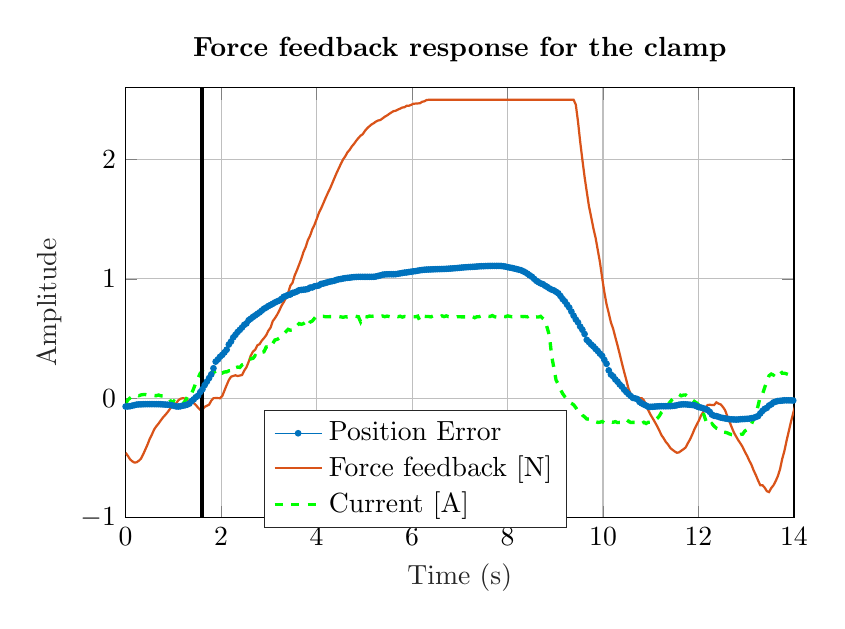
\begin{tikzpicture}

\begin{axis}[%
width=0.7\columnwidth,
height=0.45\columnwidth,
at={(2.512in,1.147in)},
scale only axis,
xmin=0,
xmax=14,
xlabel style={font=\color{white!15!black}},
xlabel={Time (s)},
ymin=-1,
ymax=2.6,
ylabel style={font=\color{white!15!black}},
ylabel={Amplitude},
axis background/.style={fill=white},
title style={font=\bfseries},
title={Force feedback response for the clamp},
xmajorgrids,
ymajorgrids,
legend style={legend cell align=left, align=left, draw=white!15!black, at={(0.66,0.25)}}
]

\addplot [color=mycolor1, draw=none, mark=*, mark size=1,mark options={solid, mycolor1}]
  table[row sep=crcr]{%
0	-0.069839\\
0.046	-0.0691929999999998\\
0.092	-0.0674169999999998\\
0.138	-0.0627580000000001\\
0.184	-0.0585599999999999\\
0.23	-0.053715\\
0.276	-0.052262\\
0.322	-0.0517779999999999\\
0.368	-0.0508089999999999\\
0.414	-0.050325\\
0.46	-0.0500019999999999\\
0.506	-0.0500019999999999\\
0.552	-0.0500019999999999\\
0.598	-0.0500019999999999\\
0.644	-0.050233\\
0.69	-0.0504629999999999\\
0.736	-0.0509360000000001\\
0.782	-0.0523979999999999\\
0.828	-0.0533170000000001\\
0.874	-0.0544640000000001\\
0.92	-0.0558380000000001\\
0.966	-0.059431\\
1.012	-0.0646089999999999\\
1.058	-0.069102\\
1.104	-0.070166\\
1.15	-0.0678619999999999\\
1.196	-0.0632820000000001\\
1.242	-0.0596559999999999\\
1.288	-0.054314\\
1.334	-0.045984\\
1.38	-0.0253700000000001\\
1.426	-0.00976399999999988\\
1.472	0.00805999999999996\\
1.518	0.0212249999999999\\
1.564	0.051482\\
1.61	0.0750869999999999\\
1.656	0.109672\\
1.702	0.138343\\
1.748	0.168177\\
1.794	0.199188\\
1.84	0.250473\\
1.886	0.306211\\
1.932	0.324103\\
1.978	0.347052\\
2.024	0.362787\\
2.07	0.383776\\
2.116	0.406007\\
2.162	0.449559\\
2.208	0.474824\\
2.254	0.508958\\
2.3	0.530804\\
2.346	0.554437\\
2.392	0.572537\\
2.438	0.591942\\
2.484	0.614258\\
2.53	0.625926\\
2.576	0.652916\\
2.622	0.665954\\
2.668	0.680707\\
2.714	0.6931054\\
2.76	0.7064931\\
2.806	0.7187228\\
2.852	0.7341136\\
2.898	0.7492224\\
2.944	0.7593239\\
2.99	0.7720971\\
3.036	0.7809118\\
3.082	0.7910974\\
3.128	0.8020223\\
3.174	0.81066\\
3.22	0.8186307\\
3.266	0.8319814\\
3.312	0.8492741\\
3.358	0.8558223\\
3.404	0.8646376\\
3.45	0.868742\\
3.496	0.8814436\\
3.542	0.8863328\\
3.588	0.8938385\\
3.634	0.9044656\\
3.68	0.9069801\\
3.726	0.9089659\\
3.772	0.9109976\\
3.818	0.9148639\\
3.864	0.9265554\\
3.91	0.9278963\\
3.956	0.9373217\\
4.002	0.940841\\
4.048	0.9445568\\
4.094	0.95726415\\
4.14	0.9604788\\
4.186	0.96597617\\
4.232	0.97119919\\
4.278	0.97641396\\
4.324	0.9801821\\
4.37	0.9838232\\
4.416	0.9907857\\
4.462	0.99572\\
4.508	0.9983443\\
4.554	1.0027004\\
4.6	1.0057562\\
4.646	1.0081051\\
4.692	1.0098843\\
4.738	1.0125273\\
4.784	1.0145615\\
4.83	1.015724\\
4.876	1.0164667\\
4.922	1.0164667\\
4.968	1.0164667\\
5.014	1.0164667\\
5.06	1.0164667\\
5.106	1.0164667\\
5.152	1.0164667\\
5.198	1.017048\\
5.244	1.0196638\\
5.29	1.0246052\\
5.336	1.0286748\\
5.382	1.0344887\\
5.428	1.0368141\\
5.474	1.0379768\\
5.52	1.0385582\\
5.566	1.0385582\\
5.612	1.0385582\\
5.658	1.0391396\\
5.704	1.0420462\\
5.75	1.045534\\
5.796	1.0490214\\
5.842	1.0522178\\
5.888	1.0536705\\
5.934	1.0571568\\
5.98	1.059633\\
6.026	1.062445\\
6.072	1.0644935\\
6.118	1.0679936\\
6.164	1.0718006\\
6.21	1.0739226\\
6.256	1.0760766\\
6.302	1.0773746\\
6.348	1.0781606\\
6.394	1.0786866\\
6.44	1.0796386\\
6.486	1.0806226\\
6.532	1.0811326\\
6.578	1.0815816\\
6.624	1.0821676\\
6.67	1.0826356\\
6.716	1.0836156\\
6.762	1.0849286\\
6.808	1.0862066\\
6.854	1.0874876\\
6.9	1.0889816\\
6.946	1.0904386\\
6.992	1.0921886\\
7.038	1.0943516\\
7.084	1.0958206\\
7.13	1.0971756\\
7.176	1.0983656\\
7.222	1.0995076\\
7.268	1.1005966\\
7.314	1.1015086\\
7.36	1.1031166\\
7.406	1.1045566\\
7.452	1.1057716\\
7.498	1.1059546\\
7.544	1.1072416\\
7.59	1.1076566\\
7.636	1.1080086\\
7.682	1.1083606\\
7.728	1.1083606\\
7.774	1.1082496\\
7.82	1.1082496\\
7.866	1.1078506\\
7.912	1.1055066\\
7.958	1.1023436\\
8.004	1.0977176\\
8.05	1.0940366\\
8.096	1.0909596\\
8.142	1.0861036\\
8.188	1.0816106\\
8.234	1.0766646\\
8.28	1.0723386\\
8.326	1.0637863\\
8.372	1.0543818\\
8.418	1.0428257\\
8.464	1.029448\\
8.51	1.0175659\\
8.556	1.0002029\\
8.602	0.9837055\\
8.648	0.97187785\\
8.694	0.96156563\\
8.74	0.9554396\\
8.786	0.942303\\
8.832	0.9318928\\
8.878	0.9191614\\
8.924	0.9095359\\
8.97	0.9029574\\
9.016	0.8912888\\
9.062	0.879097\\
9.108	0.8563865\\
9.154	0.8307516\\
9.2	0.8113894\\
9.246	0.7837317\\
9.292	0.7592755\\
9.338	0.725409\\
9.384	0.691096\\
9.43	0.659743\\
9.476	0.635184\\
9.522	0.599631\\
9.568	0.572746\\
9.614	0.537474\\
9.66	0.488529\\
9.706	0.470013\\
9.752	0.449131\\
9.798	0.434072\\
9.844	0.412879\\
9.89	0.394881\\
9.936	0.372667\\
9.982	0.354272\\
10.028	0.320757\\
10.074	0.287993\\
10.12	0.232964\\
10.166	0.197741\\
10.212	0.18275\\
10.258	0.156795\\
10.304	0.138484\\
10.35	0.114872\\
10.396	0.097008\\
10.442	0.071595\\
10.488	0.05155\\
10.534	0.034095\\
10.58	0.0179400000000001\\
10.626	0.002305\\
10.672	-0.00167099999999998\\
10.718	-0.00769699999999984\\
10.764	-0.030978\\
10.81	-0.0429710000000001\\
10.856	-0.053148\\
10.902	-0.0618189999999998\\
10.948	-0.0720810000000001\\
10.994	-0.0724389999999999\\
11.04	-0.0717700000000001\\
11.086	-0.0703040000000001\\
11.132	-0.068948\\
11.178	-0.0678830000000001\\
11.224	-0.067339\\
11.27	-0.067339\\
11.316	-0.067339\\
11.362	-0.0671580000000001\\
11.408	-0.0669960000000001\\
11.454	-0.065239\\
11.5	-0.063358\\
11.546	-0.0595410000000001\\
11.592	-0.054964\\
11.638	-0.052603\\
11.684	-0.051604\\
11.73	-0.0518610000000002\\
11.776	-0.053331\\
11.822	-0.0551919999999999\\
11.868	-0.0570810000000002\\
11.914	-0.059763\\
11.96	-0.0673490000000001\\
12.006	-0.075137\\
12.052	-0.0787260000000001\\
12.098	-0.084632\\
12.144	-0.090457\\
12.19	-0.099099\\
12.236	-0.115104\\
12.282	-0.138322\\
12.328	-0.147654\\
12.374	-0.150269\\
12.42	-0.156016\\
12.466	-0.1626\\
12.512	-0.166108\\
12.558	-0.169979\\
12.604	-0.172681\\
12.65	-0.176454\\
12.696	-0.177723\\
12.742	-0.178345\\
12.788	-0.179376\\
12.834	-0.178237\\
12.88	-0.176378\\
12.926	-0.175254\\
12.972	-0.174123\\
13.018	-0.172999\\
13.064	-0.171682\\
13.11	-0.167706\\
13.156	-0.164679\\
13.202	-0.157745\\
13.248	-0.1501\\
13.294	-0.127712\\
13.34	-0.106903\\
13.386	-0.0901689999999999\\
13.432	-0.0812360000000001\\
13.478	-0.0620539999999998\\
13.524	-0.0516510000000001\\
13.57	-0.035822\\
13.616	-0.029779\\
13.662	-0.0236429999999999\\
13.708	-0.0221900000000002\\
13.754	-0.0202520000000002\\
13.8	-0.0181120000000001\\
13.846	-0.018038\\
13.892	-0.018243\\
13.938	-0.0184470000000001\\
13.984	-0.019682\\
14.03	-0.0207010000000001\\
14.076	-0.0221230000000001\\
14.122	-0.023096\\
14.168	-0.023096\\
14.214	-0.023096\\
14.26	-0.0234529999999999\\
14.306	-0.024132\\
14.352	-0.0254239999999999\\
14.398	-0.0299449999999999\\
14.444	-0.033693\\
14.49	-0.0363100000000001\\
14.536	-0.0374399999999999\\
14.582	-0.0393779999999999\\
14.628	-0.039701\\
14.674	-0.0398689999999999\\
14.72	-0.0398770000000002\\
14.766	-0.039682\\
14.812	-0.039682\\
14.858	-0.039682\\
14.904	-0.039682\\
14.95	-0.039682\\
14.996	-0.0391299999999999\\
15.042	-0.0387390000000001\\
15.088	-0.0385439999999999\\
15.134	-0.038152\\
15.18	-0.0377609999999999\\
15.226	-0.0377609999999999\\
15.272	-0.0377609999999999\\
15.318	-0.0377609999999999\\
15.364	-0.0377609999999999\\
15.41	-0.0377609999999999\\
15.456	-0.0375649999999998\\
15.502	-0.0375649999999998\\
15.548	-0.036365\\
15.594	-0.0331220000000001\\
15.64	-0.030756\\
15.686	-0.0297510000000001\\
15.732	-0.02959\\
15.778	-0.028459\\
};
\addlegendentry{Position Error}

\addplot [color=mycolor2, thick]
  table[row sep=crcr]{%
0	-0.457965\\
0.046	-0.482939\\
0.092	-0.512125\\
0.138	-0.528618\\
0.184	-0.539522\\
0.23	-0.537151\\
0.276	-0.524402\\
0.322	-0.507127\\
0.368	-0.470289\\
0.414	-0.428809\\
0.46	-0.387254\\
0.506	-0.339716\\
0.552	-0.303282\\
0.598	-0.26139\\
0.644	-0.235044\\
0.69	-0.212801\\
0.736	-0.186553\\
0.782	-0.161903\\
0.828	-0.14172\\
0.874	-0.120005\\
0.92	-0.094566\\
0.966	-0.0684803\\
1.012	-0.0608241\\
1.058	-0.0433587\\
1.104	-0.0174891\\
1.15	-0.00521286\\
1.196	0.000178016\\
1.242	-0.00297375\\
1.288	-0.0138918\\
1.334	-0.026421\\
1.38	-0.0261145\\
1.426	-0.0405375\\
1.472	-0.0576523\\
1.518	-0.0799315\\
1.564	-0.0976721\\
1.61	-0.0951568\\
1.656	-0.0724242\\
1.702	-0.0633538\\
1.748	-0.0541451\\
1.794	-0.021039\\
1.84	0.000387498\\
1.886	0.00063466\\
1.932	0.000510842\\
1.978	1.40871e-05\\
2.024	0.0176141\\
2.07	0.0641683\\
2.116	0.109299\\
2.162	0.152024\\
2.208	0.179542\\
2.254	0.185892\\
2.3	0.191742\\
2.346	0.185386\\
2.392	0.189675\\
2.438	0.193986\\
2.484	0.230854\\
2.53	0.257935\\
2.576	0.303503\\
2.622	0.357063\\
2.668	0.390772\\
2.714	0.405952\\
2.76	0.443154\\
2.806	0.452801\\
2.852	0.481958\\
2.898	0.503039\\
2.944	0.527297\\
2.99	0.56528\\
3.036	0.591189\\
3.082	0.645425\\
3.128	0.670379\\
3.174	0.699748\\
3.22	0.735109\\
3.266	0.774628\\
3.312	0.805072\\
3.358	0.83938\\
3.404	0.882872\\
3.45	0.942162\\
3.496	0.967106\\
3.542	1.02907\\
3.588	1.07135\\
3.634	1.11914\\
3.68	1.16782\\
3.726	1.22586\\
3.772	1.26648\\
3.818	1.32544\\
3.864	1.36167\\
3.91	1.41453\\
3.956	1.45284\\
4.002	1.50118\\
4.048	1.55186\\
4.094	1.58921\\
4.14	1.63147\\
4.186	1.67488\\
4.232	1.71576\\
4.278	1.75288\\
4.324	1.79633\\
4.37	1.84079\\
4.416	1.88369\\
4.462	1.92324\\
4.508	1.96243\\
4.554	1.99936\\
4.6	2.02567\\
4.646	2.05945\\
4.692	2.08038\\
4.738	2.10928\\
4.784	2.13069\\
4.83	2.15696\\
4.876	2.17937\\
4.922	2.19947\\
4.968	2.21219\\
5.014	2.24018\\
5.06	2.26189\\
5.106	2.27821\\
5.152	2.29389\\
5.198	2.3042\\
5.244	2.31804\\
5.29	2.32692\\
5.336	2.33094\\
5.382	2.34414\\
5.428	2.35817\\
5.474	2.36845\\
5.52	2.38155\\
5.566	2.39363\\
5.612	2.40496\\
5.658	2.40824\\
5.704	2.41806\\
5.75	2.42631\\
5.796	2.4351\\
5.842	2.43808\\
5.888	2.45076\\
5.934	2.45048\\
5.98	2.45716\\
6.026	2.4668\\
6.072	2.46822\\
6.118	2.46973\\
6.164	2.47081\\
6.21	2.48353\\
6.256	2.48696\\
6.302	2.49787\\
6.348	2.5\\
6.394	2.5\\
6.44	2.5\\
6.486	2.5\\
6.532	2.49992\\
6.578	2.5\\
6.624	2.5\\
6.67	2.5\\
6.716	2.5\\
6.762	2.5\\
6.808	2.5\\
6.854	2.5\\
6.9	2.5\\
6.946	2.5\\
6.992	2.5\\
7.038	2.5\\
7.084	2.5\\
7.13	2.5\\
7.176	2.5\\
7.222	2.5\\
7.268	2.5\\
7.314	2.5\\
7.36	2.5\\
7.406	2.5\\
7.452	2.5\\
7.498	2.5\\
7.544	2.5\\
7.59	2.5\\
7.636	2.5\\
7.682	2.5\\
7.728	2.5\\
7.774	2.5\\
7.82	2.5\\
7.866	2.5\\
7.912	2.5\\
7.958	2.5\\
8.004	2.5\\
8.05	2.5\\
8.096	2.5\\
8.142	2.5\\
8.188	2.5\\
8.234	2.5\\
8.28	2.5\\
8.326	2.5\\
8.372	2.5\\
8.418	2.5\\
8.464	2.5\\
8.51	2.5\\
8.556	2.5\\
8.602	2.5\\
8.648	2.5\\
8.694	2.5\\
8.74	2.5\\
8.786	2.5\\
8.832	2.5\\
8.878	2.5\\
8.924	2.5\\
8.97	2.5\\
9.016	2.5\\
9.062	2.5\\
9.108	2.5\\
9.154	2.5\\
9.2	2.5\\
9.246	2.5\\
9.292	2.5\\
9.338	2.5\\
9.384	2.5\\
9.43	2.45972\\
9.476	2.31758\\
9.522	2.14825\\
9.568	1.99722\\
9.614	1.85379\\
9.66	1.72876\\
9.706	1.60717\\
9.752	1.51777\\
9.798	1.42349\\
9.844	1.34486\\
9.89	1.24209\\
9.936	1.13853\\
9.982	1.0087\\
10.028	0.888403\\
10.074	0.786921\\
10.12	0.712798\\
10.166	0.633521\\
10.212	0.58201\\
10.258	0.510575\\
10.304	0.442393\\
10.35	0.369444\\
10.396	0.293081\\
10.442	0.220909\\
10.488	0.152474\\
10.534	0.078849\\
10.58	0.0342911\\
10.626	0.000124028\\
10.672	0.000301921\\
10.718	0.000252726\\
10.764	0.000330059\\
10.81	0.000273753\\
10.856	-0.0174561\\
10.902	-0.0569983\\
10.948	-0.101156\\
10.994	-0.137496\\
11.04	-0.16853\\
11.086	-0.20015\\
11.132	-0.233028\\
11.178	-0.269616\\
11.224	-0.309738\\
11.27	-0.335806\\
11.316	-0.366884\\
11.362	-0.387696\\
11.408	-0.416516\\
11.454	-0.432208\\
11.5	-0.445834\\
11.546	-0.45736\\
11.592	-0.45423\\
11.638	-0.440815\\
11.684	-0.428176\\
11.73	-0.413655\\
11.776	-0.377847\\
11.822	-0.346186\\
11.868	-0.30626\\
11.914	-0.261468\\
11.96	-0.224553\\
12.006	-0.188972\\
12.052	-0.146403\\
12.098	-0.116957\\
12.144	-0.0867584\\
12.19	-0.0573152\\
12.236	-0.0552171\\
12.282	-0.0574377\\
12.328	-0.0575676\\
12.374	-0.0349744\\
12.42	-0.046042\\
12.466	-0.0523814\\
12.512	-0.0740595\\
12.558	-0.101582\\
12.604	-0.151553\\
12.65	-0.197503\\
12.696	-0.243833\\
12.742	-0.288091\\
12.788	-0.321104\\
12.834	-0.352334\\
12.88	-0.379869\\
12.926	-0.410188\\
12.972	-0.449443\\
13.018	-0.483054\\
13.064	-0.523156\\
13.11	-0.558781\\
13.156	-0.606164\\
13.202	-0.644778\\
13.248	-0.689715\\
13.294	-0.72931\\
13.34	-0.729152\\
13.386	-0.749485\\
13.432	-0.779093\\
13.478	-0.786947\\
13.524	-0.753038\\
13.57	-0.730523\\
13.616	-0.695568\\
13.662	-0.65353\\
13.708	-0.595233\\
13.754	-0.50868\\
13.8	-0.441981\\
13.846	-0.355192\\
13.892	-0.275813\\
13.938	-0.196536\\
13.984	-0.125382\\
14.03	-0.0564939\\
14.076	0.000372308\\
14.122	0.000553329\\
14.168	0.000643569\\
14.214	0.000462548\\
14.26	0.00539057\\
14.306	0.0388688\\
14.352	0.0787901\\
14.398	0.106753\\
14.444	0.130374\\
14.49	0.152278\\
14.536	0.170294\\
14.582	0.159808\\
14.628	0.155049\\
14.674	0.143513\\
14.72	0.12149\\
14.766	0.0911616\\
14.812	0.0673271\\
14.858	0.0494943\\
14.904	0.0241393\\
14.95	0.00996927\\
14.996	0.000383604\\
15.042	1.06228e-05\\
15.088	0.000199578\\
15.134	0.00057731\\
15.18	0.000486604\\
15.226	0.000296169\\
15.272	0.000202064\\
15.318	0.000297389\\
15.364	0.000202064\\
15.41	0.000297389\\
15.456	0.000682615\\
15.502	0.000490612\\
15.548	0.000398122\\
15.594	0.00049462\\
15.64	0.000399735\\
15.686	0.000596488\\
15.732	0.000108347\\
15.778	0.000401348\\
};
\addlegendentry{Force feedback [N]}

\addplot [color=green, dashed, very thick]
  table[row sep=crcr]{%
0	-0.0462933\\
0.046	-0.0146618\\
0.092	0.00131416\\
0.138	0.0156918\\
0.184	0.0268745\\
0.23	0.0278339\\
0.276	0.0204849\\
0.322	0.027195\\
0.368	0.0300694\\
0.414	0.0303898\\
0.46	0.026556\\
0.506	0.0262356\\
0.552	0.0275135\\
0.598	0.0217628\\
0.644	0.0211239\\
0.69	0.026556\\
0.736	0.0195255\\
0.782	0.0188866\\
0.828	0.0115376\\
0.874	-0.00220108\\
0.92	-0.00891113\\
0.966	-0.0418205\\
1.012	-0.0236073\\
1.058	-0.0344715\\
1.104	-0.0450153\\
1.15	-0.0504456\\
1.196	-0.0485287\\
1.242	-0.0261631\\
1.288	0.0057869\\
1.334	0.0434895\\
1.38	0.0380573\\
1.426	0.081192\\
1.472	0.129118\\
1.518	0.168417\\
1.564	0.209953\\
1.61	0.222414\\
1.656	0.213787\\
1.702	0.216024\\
1.748	0.229124\\
1.794	0.210911\\
1.84	0.235514\\
1.886	0.200048\\
1.932	0.214746\\
1.978	0.216024\\
2.024	0.209953\\
2.07	0.219858\\
2.116	0.220497\\
2.162	0.229124\\
2.208	0.231041\\
2.254	0.261074\\
2.3	0.255003\\
2.346	0.260756\\
2.392	0.25724\\
2.438	0.278328\\
2.484	0.286955\\
2.53	0.301332\\
2.576	0.316988\\
2.622	0.329769\\
2.668	0.333603\\
2.714	0.356928\\
2.76	0.346703\\
2.806	0.368429\\
2.852	0.383766\\
2.898	0.388559\\
2.944	0.428497\\
2.99	0.431053\\
3.036	0.468117\\
3.082	0.458851\\
3.128	0.487926\\
3.174	0.492718\\
3.22	0.502623\\
3.266	0.524349\\
3.312	0.540007\\
3.358	0.557259\\
3.404	0.57675\\
3.45	0.56908\\
3.496	0.571957\\
3.542	0.575151\\
3.588	0.605825\\
3.634	0.625315\\
3.68	0.618925\\
3.726	0.624355\\
3.772	0.636816\\
3.818	0.607422\\
3.864	0.637775\\
3.91	0.646082\\
3.956	0.668768\\
4.002	0.687618\\
4.048	0.682827\\
4.094	0.686979\\
4.14	0.686022\\
4.186	0.682186\\
4.232	0.681547\\
4.278	0.683466\\
4.324	0.682507\\
4.37	0.681868\\
4.416	0.682827\\
4.462	0.684423\\
4.508	0.681547\\
4.554	0.677713\\
4.6	0.681868\\
4.646	0.680908\\
4.692	0.685062\\
4.738	0.685383\\
4.784	0.690174\\
4.83	0.685383\\
4.876	0.682507\\
4.922	0.640331\\
4.968	0.684105\\
5.014	0.683466\\
5.06	0.681229\\
5.106	0.687939\\
5.152	0.685701\\
5.198	0.688257\\
5.244	0.681229\\
5.29	0.679312\\
5.336	0.684744\\
5.382	0.688896\\
5.428	0.682827\\
5.474	0.687618\\
5.52	0.684105\\
5.566	0.67963\\
5.612	0.678034\\
5.658	0.687939\\
5.704	0.682507\\
5.75	0.686661\\
5.796	0.678991\\
5.842	0.684744\\
5.888	0.681868\\
5.934	0.685701\\
5.98	0.687939\\
6.026	0.681868\\
6.072	0.681868\\
6.118	0.687618\\
6.164	0.648638\\
6.21	0.681229\\
6.256	0.685701\\
6.302	0.684423\\
6.348	0.683784\\
6.394	0.681229\\
6.44	0.688578\\
6.486	0.681868\\
6.532	0.682186\\
6.578	0.68059\\
6.624	0.689856\\
6.67	0.683466\\
6.716	0.689856\\
6.762	0.682827\\
6.808	0.681229\\
6.854	0.680908\\
6.9	0.676756\\
6.946	0.682507\\
6.992	0.682827\\
7.038	0.680908\\
7.084	0.681229\\
7.13	0.68059\\
7.176	0.687939\\
7.222	0.678352\\
7.268	0.682827\\
7.314	0.6742\\
7.36	0.682827\\
7.406	0.682827\\
7.452	0.690174\\
7.498	0.681547\\
7.544	0.686979\\
7.59	0.685383\\
7.636	0.684744\\
7.682	0.692091\\
7.728	0.682186\\
7.774	0.678673\\
7.82	0.684744\\
7.866	0.692091\\
7.912	0.685383\\
7.958	0.682827\\
8.004	0.689535\\
8.05	0.685383\\
8.096	0.681547\\
8.142	0.683146\\
8.188	0.679951\\
8.234	0.682186\\
8.28	0.683784\\
8.326	0.683466\\
8.372	0.683784\\
8.418	0.681547\\
8.464	0.69273\\
8.51	0.680269\\
8.556	0.678034\\
8.602	0.680908\\
8.648	0.67963\\
8.694	0.685701\\
8.74	0.667809\\
8.786	0.65439\\
8.832	0.587612\\
8.878	0.522753\\
8.924	0.353092\\
8.97	0.255323\\
9.016	0.151484\\
9.062	0.117296\\
9.108	0.0735226\\
9.154	0.0380573\\
9.2	0.0124969\\
9.246	-0.00699234\\
9.292	-0.0335121\\
9.338	-0.043417\\
9.384	-0.0552387\\
9.43	-0.0792027\\
9.476	-0.110834\\
9.522	-0.115625\\
9.568	-0.141827\\
9.614	-0.156843\\
9.66	-0.174736\\
9.706	-0.176014\\
9.752	-0.183681\\
9.798	-0.182404\\
9.844	-0.197102\\
9.89	-0.203171\\
9.936	-0.201254\\
9.982	-0.195503\\
10.028	-0.207645\\
10.074	-0.211479\\
10.12	-0.208923\\
10.166	-0.199337\\
10.212	-0.202213\\
10.258	-0.196781\\
10.304	-0.204449\\
10.35	-0.202852\\
10.396	-0.202213\\
10.442	-0.209881\\
10.488	-0.214354\\
10.534	-0.191988\\
10.58	-0.20381\\
10.626	-0.202532\\
10.672	-0.203171\\
10.718	-0.208284\\
10.764	-0.21755\\
10.81	-0.212437\\
10.856	-0.201574\\
10.902	-0.212118\\
10.948	-0.202532\\
10.994	-0.201893\\
11.04	-0.190392\\
11.086	-0.184641\\
11.132	-0.171221\\
11.178	-0.150454\\
11.224	-0.119141\\
11.27	-0.100929\\
11.316	-0.0760078\\
11.362	-0.0552387\\
11.408	-0.0299988\\
11.454	-0.0085907\\
11.5	0.00866318\\
11.546	0.0224018\\
11.592	0.0313473\\
11.638	0.019846\\
11.684	0.0259171\\
11.73	0.027195\\
11.776	0.011219\\
11.822	0.00866318\\
11.868	-0.0140228\\
11.914	-0.0271225\\
11.96	-0.0399017\\
12.006	-0.058115\\
12.052	-0.0986919\\
12.098	-0.1201\\
12.144	-0.177292\\
12.19	-0.223619\\
12.236	-0.228094\\
12.282	-0.213715\\
12.328	-0.234484\\
12.374	-0.251417\\
12.42	-0.258127\\
12.466	-0.280811\\
12.512	-0.283369\\
12.558	-0.285925\\
12.604	-0.290716\\
12.65	-0.299664\\
12.696	-0.305414\\
12.742	-0.307331\\
12.788	-0.305414\\
12.834	-0.309568\\
12.88	-0.303177\\
12.926	-0.30126\\
12.972	-0.274742\\
13.018	-0.263878\\
13.064	-0.237679\\
13.11	-0.216272\\
13.156	-0.174736\\
13.202	-0.137352\\
13.248	-0.0641861\\
13.294	0.0150528\\
13.34	0.0339031\\
13.386	0.0882206\\
13.432	0.139662\\
13.478	0.188227\\
13.524	0.202286\\
13.57	0.193338\\
13.616	0.21826\\
13.662	0.226248\\
13.708	0.234556\\
13.754	0.208355\\
13.8	0.208994\\
13.846	0.203243\\
13.892	0.196533\\
13.938	0.189505\\
13.984	0.18631\\
14.03	0.17321\\
14.076	0.157873\\
14.122	0.146051\\
14.168	0.111225\\
14.214	0.0952492\\
14.26	0.0613823\\
14.306	0.0450859\\
14.352	0.0188866\\
14.398	-0.00571442\\
14.444	-0.0213718\\
14.49	-0.0296783\\
14.536	-0.0402222\\
14.582	-0.0309563\\
14.628	-0.0306377\\
14.674	-0.036068\\
14.72	-0.0379848\\
14.766	-0.0357494\\
14.812	-0.0312767\\
14.858	-0.0383053\\
14.904	-0.0303173\\
14.95	-0.0306377\\
14.996	-0.0296783\\
15.042	-0.0216904\\
15.088	-0.0216904\\
15.134	-0.0137024\\
15.18	0.000675201\\
15.226	-0.00251961\\
15.272	0.0124969\\
15.318	0.0131359\\
15.364	0.0211239\\
15.41	0.0255966\\
15.456	0.0287914\\
15.502	0.0310287\\
15.548	0.0326252\\
15.594	0.0262356\\
15.64	0.0294304\\
15.686	0.0422115\\
15.732	0.0479622\\
15.778	0.0447674\\
};
\addlegendentry{Current [A]}
\addplot [color=black, forget plot, very thick]
  table[row sep=crcr]{%
1.6	-1\\
1.6	2.6\\
};
\end{axis}
\end{tikzpicture}%
\end{figure}
\end{frame}

\begin{frame}<beamer>
\vspace*{1.5cm}
\begin{figure}
\centering
% This file was created by matlab2tikz.
%
%The latest updates can be retrieved from
%  http://www.mathworks.com/matlabcentral/fileexchange/22022-matlab2tikz-matlab2tikz
%where you can also make suggestions and rate matlab2tikz.
%
\definecolor{mycolor1}{rgb}{0.00000,0.44700,0.74100}%
\definecolor{mycolor2}{rgb}{0.85000,0.32500,0.09800}%
%
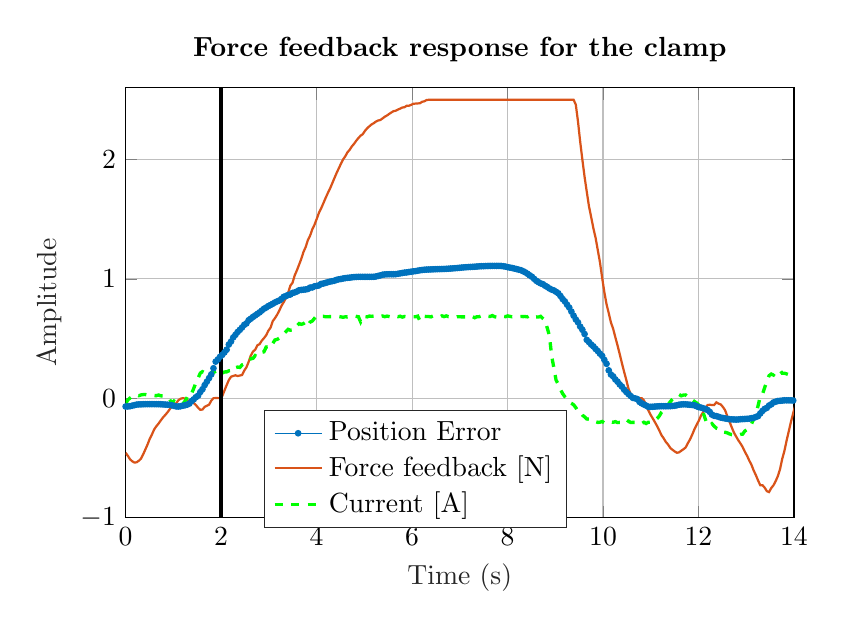
\begin{tikzpicture}

\begin{axis}[%
width=0.7\columnwidth,
height=0.45\columnwidth,
at={(2.512in,1.147in)},
scale only axis,
xmin=0,
xmax=14,
xlabel style={font=\color{white!15!black}},
xlabel={Time (s)},
ymin=-1,
ymax=2.6,
ylabel style={font=\color{white!15!black}},
ylabel={Amplitude},
axis background/.style={fill=white},
title style={font=\bfseries},
title={Force feedback response for the clamp},
xmajorgrids,
ymajorgrids,
legend style={legend cell align=left, align=left, draw=white!15!black, at={(0.66,0.25)}}
]

\addplot [color=mycolor1, draw=none, mark=*, mark size=1,mark options={solid, mycolor1}]
  table[row sep=crcr]{%
0	-0.069839\\
0.046	-0.0691929999999998\\
0.092	-0.0674169999999998\\
0.138	-0.0627580000000001\\
0.184	-0.0585599999999999\\
0.23	-0.053715\\
0.276	-0.052262\\
0.322	-0.0517779999999999\\
0.368	-0.0508089999999999\\
0.414	-0.050325\\
0.46	-0.0500019999999999\\
0.506	-0.0500019999999999\\
0.552	-0.0500019999999999\\
0.598	-0.0500019999999999\\
0.644	-0.050233\\
0.69	-0.0504629999999999\\
0.736	-0.0509360000000001\\
0.782	-0.0523979999999999\\
0.828	-0.0533170000000001\\
0.874	-0.0544640000000001\\
0.92	-0.0558380000000001\\
0.966	-0.059431\\
1.012	-0.0646089999999999\\
1.058	-0.069102\\
1.104	-0.070166\\
1.15	-0.0678619999999999\\
1.196	-0.0632820000000001\\
1.242	-0.0596559999999999\\
1.288	-0.054314\\
1.334	-0.045984\\
1.38	-0.0253700000000001\\
1.426	-0.00976399999999988\\
1.472	0.00805999999999996\\
1.518	0.0212249999999999\\
1.564	0.051482\\
1.61	0.0750869999999999\\
1.656	0.109672\\
1.702	0.138343\\
1.748	0.168177\\
1.794	0.199188\\
1.84	0.250473\\
1.886	0.306211\\
1.932	0.324103\\
1.978	0.347052\\
2.024	0.362787\\
2.07	0.383776\\
2.116	0.406007\\
2.162	0.449559\\
2.208	0.474824\\
2.254	0.508958\\
2.3	0.530804\\
2.346	0.554437\\
2.392	0.572537\\
2.438	0.591942\\
2.484	0.614258\\
2.53	0.625926\\
2.576	0.652916\\
2.622	0.665954\\
2.668	0.680707\\
2.714	0.6931054\\
2.76	0.7064931\\
2.806	0.7187228\\
2.852	0.7341136\\
2.898	0.7492224\\
2.944	0.7593239\\
2.99	0.7720971\\
3.036	0.7809118\\
3.082	0.7910974\\
3.128	0.8020223\\
3.174	0.81066\\
3.22	0.8186307\\
3.266	0.8319814\\
3.312	0.8492741\\
3.358	0.8558223\\
3.404	0.8646376\\
3.45	0.868742\\
3.496	0.8814436\\
3.542	0.8863328\\
3.588	0.8938385\\
3.634	0.9044656\\
3.68	0.9069801\\
3.726	0.9089659\\
3.772	0.9109976\\
3.818	0.9148639\\
3.864	0.9265554\\
3.91	0.9278963\\
3.956	0.9373217\\
4.002	0.940841\\
4.048	0.9445568\\
4.094	0.95726415\\
4.14	0.9604788\\
4.186	0.96597617\\
4.232	0.97119919\\
4.278	0.97641396\\
4.324	0.9801821\\
4.37	0.9838232\\
4.416	0.9907857\\
4.462	0.99572\\
4.508	0.9983443\\
4.554	1.0027004\\
4.6	1.0057562\\
4.646	1.0081051\\
4.692	1.0098843\\
4.738	1.0125273\\
4.784	1.0145615\\
4.83	1.015724\\
4.876	1.0164667\\
4.922	1.0164667\\
4.968	1.0164667\\
5.014	1.0164667\\
5.06	1.0164667\\
5.106	1.0164667\\
5.152	1.0164667\\
5.198	1.017048\\
5.244	1.0196638\\
5.29	1.0246052\\
5.336	1.0286748\\
5.382	1.0344887\\
5.428	1.0368141\\
5.474	1.0379768\\
5.52	1.0385582\\
5.566	1.0385582\\
5.612	1.0385582\\
5.658	1.0391396\\
5.704	1.0420462\\
5.75	1.045534\\
5.796	1.0490214\\
5.842	1.0522178\\
5.888	1.0536705\\
5.934	1.0571568\\
5.98	1.059633\\
6.026	1.062445\\
6.072	1.0644935\\
6.118	1.0679936\\
6.164	1.0718006\\
6.21	1.0739226\\
6.256	1.0760766\\
6.302	1.0773746\\
6.348	1.0781606\\
6.394	1.0786866\\
6.44	1.0796386\\
6.486	1.0806226\\
6.532	1.0811326\\
6.578	1.0815816\\
6.624	1.0821676\\
6.67	1.0826356\\
6.716	1.0836156\\
6.762	1.0849286\\
6.808	1.0862066\\
6.854	1.0874876\\
6.9	1.0889816\\
6.946	1.0904386\\
6.992	1.0921886\\
7.038	1.0943516\\
7.084	1.0958206\\
7.13	1.0971756\\
7.176	1.0983656\\
7.222	1.0995076\\
7.268	1.1005966\\
7.314	1.1015086\\
7.36	1.1031166\\
7.406	1.1045566\\
7.452	1.1057716\\
7.498	1.1059546\\
7.544	1.1072416\\
7.59	1.1076566\\
7.636	1.1080086\\
7.682	1.1083606\\
7.728	1.1083606\\
7.774	1.1082496\\
7.82	1.1082496\\
7.866	1.1078506\\
7.912	1.1055066\\
7.958	1.1023436\\
8.004	1.0977176\\
8.05	1.0940366\\
8.096	1.0909596\\
8.142	1.0861036\\
8.188	1.0816106\\
8.234	1.0766646\\
8.28	1.0723386\\
8.326	1.0637863\\
8.372	1.0543818\\
8.418	1.0428257\\
8.464	1.029448\\
8.51	1.0175659\\
8.556	1.0002029\\
8.602	0.9837055\\
8.648	0.97187785\\
8.694	0.96156563\\
8.74	0.9554396\\
8.786	0.942303\\
8.832	0.9318928\\
8.878	0.9191614\\
8.924	0.9095359\\
8.97	0.9029574\\
9.016	0.8912888\\
9.062	0.879097\\
9.108	0.8563865\\
9.154	0.8307516\\
9.2	0.8113894\\
9.246	0.7837317\\
9.292	0.7592755\\
9.338	0.725409\\
9.384	0.691096\\
9.43	0.659743\\
9.476	0.635184\\
9.522	0.599631\\
9.568	0.572746\\
9.614	0.537474\\
9.66	0.488529\\
9.706	0.470013\\
9.752	0.449131\\
9.798	0.434072\\
9.844	0.412879\\
9.89	0.394881\\
9.936	0.372667\\
9.982	0.354272\\
10.028	0.320757\\
10.074	0.287993\\
10.12	0.232964\\
10.166	0.197741\\
10.212	0.18275\\
10.258	0.156795\\
10.304	0.138484\\
10.35	0.114872\\
10.396	0.097008\\
10.442	0.071595\\
10.488	0.05155\\
10.534	0.034095\\
10.58	0.0179400000000001\\
10.626	0.002305\\
10.672	-0.00167099999999998\\
10.718	-0.00769699999999984\\
10.764	-0.030978\\
10.81	-0.0429710000000001\\
10.856	-0.053148\\
10.902	-0.0618189999999998\\
10.948	-0.0720810000000001\\
10.994	-0.0724389999999999\\
11.04	-0.0717700000000001\\
11.086	-0.0703040000000001\\
11.132	-0.068948\\
11.178	-0.0678830000000001\\
11.224	-0.067339\\
11.27	-0.067339\\
11.316	-0.067339\\
11.362	-0.0671580000000001\\
11.408	-0.0669960000000001\\
11.454	-0.065239\\
11.5	-0.063358\\
11.546	-0.0595410000000001\\
11.592	-0.054964\\
11.638	-0.052603\\
11.684	-0.051604\\
11.73	-0.0518610000000002\\
11.776	-0.053331\\
11.822	-0.0551919999999999\\
11.868	-0.0570810000000002\\
11.914	-0.059763\\
11.96	-0.0673490000000001\\
12.006	-0.075137\\
12.052	-0.0787260000000001\\
12.098	-0.084632\\
12.144	-0.090457\\
12.19	-0.099099\\
12.236	-0.115104\\
12.282	-0.138322\\
12.328	-0.147654\\
12.374	-0.150269\\
12.42	-0.156016\\
12.466	-0.1626\\
12.512	-0.166108\\
12.558	-0.169979\\
12.604	-0.172681\\
12.65	-0.176454\\
12.696	-0.177723\\
12.742	-0.178345\\
12.788	-0.179376\\
12.834	-0.178237\\
12.88	-0.176378\\
12.926	-0.175254\\
12.972	-0.174123\\
13.018	-0.172999\\
13.064	-0.171682\\
13.11	-0.167706\\
13.156	-0.164679\\
13.202	-0.157745\\
13.248	-0.1501\\
13.294	-0.127712\\
13.34	-0.106903\\
13.386	-0.0901689999999999\\
13.432	-0.0812360000000001\\
13.478	-0.0620539999999998\\
13.524	-0.0516510000000001\\
13.57	-0.035822\\
13.616	-0.029779\\
13.662	-0.0236429999999999\\
13.708	-0.0221900000000002\\
13.754	-0.0202520000000002\\
13.8	-0.0181120000000001\\
13.846	-0.018038\\
13.892	-0.018243\\
13.938	-0.0184470000000001\\
13.984	-0.019682\\
14.03	-0.0207010000000001\\
14.076	-0.0221230000000001\\
14.122	-0.023096\\
14.168	-0.023096\\
14.214	-0.023096\\
14.26	-0.0234529999999999\\
14.306	-0.024132\\
14.352	-0.0254239999999999\\
14.398	-0.0299449999999999\\
14.444	-0.033693\\
14.49	-0.0363100000000001\\
14.536	-0.0374399999999999\\
14.582	-0.0393779999999999\\
14.628	-0.039701\\
14.674	-0.0398689999999999\\
14.72	-0.0398770000000002\\
14.766	-0.039682\\
14.812	-0.039682\\
14.858	-0.039682\\
14.904	-0.039682\\
14.95	-0.039682\\
14.996	-0.0391299999999999\\
15.042	-0.0387390000000001\\
15.088	-0.0385439999999999\\
15.134	-0.038152\\
15.18	-0.0377609999999999\\
15.226	-0.0377609999999999\\
15.272	-0.0377609999999999\\
15.318	-0.0377609999999999\\
15.364	-0.0377609999999999\\
15.41	-0.0377609999999999\\
15.456	-0.0375649999999998\\
15.502	-0.0375649999999998\\
15.548	-0.036365\\
15.594	-0.0331220000000001\\
15.64	-0.030756\\
15.686	-0.0297510000000001\\
15.732	-0.02959\\
15.778	-0.028459\\
};
\addlegendentry{Position Error}

\addplot [color=mycolor2, thick]
  table[row sep=crcr]{%
0	-0.457965\\
0.046	-0.482939\\
0.092	-0.512125\\
0.138	-0.528618\\
0.184	-0.539522\\
0.23	-0.537151\\
0.276	-0.524402\\
0.322	-0.507127\\
0.368	-0.470289\\
0.414	-0.428809\\
0.46	-0.387254\\
0.506	-0.339716\\
0.552	-0.303282\\
0.598	-0.26139\\
0.644	-0.235044\\
0.69	-0.212801\\
0.736	-0.186553\\
0.782	-0.161903\\
0.828	-0.14172\\
0.874	-0.120005\\
0.92	-0.094566\\
0.966	-0.0684803\\
1.012	-0.0608241\\
1.058	-0.0433587\\
1.104	-0.0174891\\
1.15	-0.00521286\\
1.196	0.000178016\\
1.242	-0.00297375\\
1.288	-0.0138918\\
1.334	-0.026421\\
1.38	-0.0261145\\
1.426	-0.0405375\\
1.472	-0.0576523\\
1.518	-0.0799315\\
1.564	-0.0976721\\
1.61	-0.0951568\\
1.656	-0.0724242\\
1.702	-0.0633538\\
1.748	-0.0541451\\
1.794	-0.021039\\
1.84	0.000387498\\
1.886	0.00063466\\
1.932	0.000510842\\
1.978	1.40871e-05\\
2.024	0.0176141\\
2.07	0.0641683\\
2.116	0.109299\\
2.162	0.152024\\
2.208	0.179542\\
2.254	0.185892\\
2.3	0.191742\\
2.346	0.185386\\
2.392	0.189675\\
2.438	0.193986\\
2.484	0.230854\\
2.53	0.257935\\
2.576	0.303503\\
2.622	0.357063\\
2.668	0.390772\\
2.714	0.405952\\
2.76	0.443154\\
2.806	0.452801\\
2.852	0.481958\\
2.898	0.503039\\
2.944	0.527297\\
2.99	0.56528\\
3.036	0.591189\\
3.082	0.645425\\
3.128	0.670379\\
3.174	0.699748\\
3.22	0.735109\\
3.266	0.774628\\
3.312	0.805072\\
3.358	0.83938\\
3.404	0.882872\\
3.45	0.942162\\
3.496	0.967106\\
3.542	1.02907\\
3.588	1.07135\\
3.634	1.11914\\
3.68	1.16782\\
3.726	1.22586\\
3.772	1.26648\\
3.818	1.32544\\
3.864	1.36167\\
3.91	1.41453\\
3.956	1.45284\\
4.002	1.50118\\
4.048	1.55186\\
4.094	1.58921\\
4.14	1.63147\\
4.186	1.67488\\
4.232	1.71576\\
4.278	1.75288\\
4.324	1.79633\\
4.37	1.84079\\
4.416	1.88369\\
4.462	1.92324\\
4.508	1.96243\\
4.554	1.99936\\
4.6	2.02567\\
4.646	2.05945\\
4.692	2.08038\\
4.738	2.10928\\
4.784	2.13069\\
4.83	2.15696\\
4.876	2.17937\\
4.922	2.19947\\
4.968	2.21219\\
5.014	2.24018\\
5.06	2.26189\\
5.106	2.27821\\
5.152	2.29389\\
5.198	2.3042\\
5.244	2.31804\\
5.29	2.32692\\
5.336	2.33094\\
5.382	2.34414\\
5.428	2.35817\\
5.474	2.36845\\
5.52	2.38155\\
5.566	2.39363\\
5.612	2.40496\\
5.658	2.40824\\
5.704	2.41806\\
5.75	2.42631\\
5.796	2.4351\\
5.842	2.43808\\
5.888	2.45076\\
5.934	2.45048\\
5.98	2.45716\\
6.026	2.4668\\
6.072	2.46822\\
6.118	2.46973\\
6.164	2.47081\\
6.21	2.48353\\
6.256	2.48696\\
6.302	2.49787\\
6.348	2.5\\
6.394	2.5\\
6.44	2.5\\
6.486	2.5\\
6.532	2.49992\\
6.578	2.5\\
6.624	2.5\\
6.67	2.5\\
6.716	2.5\\
6.762	2.5\\
6.808	2.5\\
6.854	2.5\\
6.9	2.5\\
6.946	2.5\\
6.992	2.5\\
7.038	2.5\\
7.084	2.5\\
7.13	2.5\\
7.176	2.5\\
7.222	2.5\\
7.268	2.5\\
7.314	2.5\\
7.36	2.5\\
7.406	2.5\\
7.452	2.5\\
7.498	2.5\\
7.544	2.5\\
7.59	2.5\\
7.636	2.5\\
7.682	2.5\\
7.728	2.5\\
7.774	2.5\\
7.82	2.5\\
7.866	2.5\\
7.912	2.5\\
7.958	2.5\\
8.004	2.5\\
8.05	2.5\\
8.096	2.5\\
8.142	2.5\\
8.188	2.5\\
8.234	2.5\\
8.28	2.5\\
8.326	2.5\\
8.372	2.5\\
8.418	2.5\\
8.464	2.5\\
8.51	2.5\\
8.556	2.5\\
8.602	2.5\\
8.648	2.5\\
8.694	2.5\\
8.74	2.5\\
8.786	2.5\\
8.832	2.5\\
8.878	2.5\\
8.924	2.5\\
8.97	2.5\\
9.016	2.5\\
9.062	2.5\\
9.108	2.5\\
9.154	2.5\\
9.2	2.5\\
9.246	2.5\\
9.292	2.5\\
9.338	2.5\\
9.384	2.5\\
9.43	2.45972\\
9.476	2.31758\\
9.522	2.14825\\
9.568	1.99722\\
9.614	1.85379\\
9.66	1.72876\\
9.706	1.60717\\
9.752	1.51777\\
9.798	1.42349\\
9.844	1.34486\\
9.89	1.24209\\
9.936	1.13853\\
9.982	1.0087\\
10.028	0.888403\\
10.074	0.786921\\
10.12	0.712798\\
10.166	0.633521\\
10.212	0.58201\\
10.258	0.510575\\
10.304	0.442393\\
10.35	0.369444\\
10.396	0.293081\\
10.442	0.220909\\
10.488	0.152474\\
10.534	0.078849\\
10.58	0.0342911\\
10.626	0.000124028\\
10.672	0.000301921\\
10.718	0.000252726\\
10.764	0.000330059\\
10.81	0.000273753\\
10.856	-0.0174561\\
10.902	-0.0569983\\
10.948	-0.101156\\
10.994	-0.137496\\
11.04	-0.16853\\
11.086	-0.20015\\
11.132	-0.233028\\
11.178	-0.269616\\
11.224	-0.309738\\
11.27	-0.335806\\
11.316	-0.366884\\
11.362	-0.387696\\
11.408	-0.416516\\
11.454	-0.432208\\
11.5	-0.445834\\
11.546	-0.45736\\
11.592	-0.45423\\
11.638	-0.440815\\
11.684	-0.428176\\
11.73	-0.413655\\
11.776	-0.377847\\
11.822	-0.346186\\
11.868	-0.30626\\
11.914	-0.261468\\
11.96	-0.224553\\
12.006	-0.188972\\
12.052	-0.146403\\
12.098	-0.116957\\
12.144	-0.0867584\\
12.19	-0.0573152\\
12.236	-0.0552171\\
12.282	-0.0574377\\
12.328	-0.0575676\\
12.374	-0.0349744\\
12.42	-0.046042\\
12.466	-0.0523814\\
12.512	-0.0740595\\
12.558	-0.101582\\
12.604	-0.151553\\
12.65	-0.197503\\
12.696	-0.243833\\
12.742	-0.288091\\
12.788	-0.321104\\
12.834	-0.352334\\
12.88	-0.379869\\
12.926	-0.410188\\
12.972	-0.449443\\
13.018	-0.483054\\
13.064	-0.523156\\
13.11	-0.558781\\
13.156	-0.606164\\
13.202	-0.644778\\
13.248	-0.689715\\
13.294	-0.72931\\
13.34	-0.729152\\
13.386	-0.749485\\
13.432	-0.779093\\
13.478	-0.786947\\
13.524	-0.753038\\
13.57	-0.730523\\
13.616	-0.695568\\
13.662	-0.65353\\
13.708	-0.595233\\
13.754	-0.50868\\
13.8	-0.441981\\
13.846	-0.355192\\
13.892	-0.275813\\
13.938	-0.196536\\
13.984	-0.125382\\
14.03	-0.0564939\\
14.076	0.000372308\\
14.122	0.000553329\\
14.168	0.000643569\\
14.214	0.000462548\\
14.26	0.00539057\\
14.306	0.0388688\\
14.352	0.0787901\\
14.398	0.106753\\
14.444	0.130374\\
14.49	0.152278\\
14.536	0.170294\\
14.582	0.159808\\
14.628	0.155049\\
14.674	0.143513\\
14.72	0.12149\\
14.766	0.0911616\\
14.812	0.0673271\\
14.858	0.0494943\\
14.904	0.0241393\\
14.95	0.00996927\\
14.996	0.000383604\\
15.042	1.06228e-05\\
15.088	0.000199578\\
15.134	0.00057731\\
15.18	0.000486604\\
15.226	0.000296169\\
15.272	0.000202064\\
15.318	0.000297389\\
15.364	0.000202064\\
15.41	0.000297389\\
15.456	0.000682615\\
15.502	0.000490612\\
15.548	0.000398122\\
15.594	0.00049462\\
15.64	0.000399735\\
15.686	0.000596488\\
15.732	0.000108347\\
15.778	0.000401348\\
};
\addlegendentry{Force feedback [N]}

\addplot [color=green, dashed, very thick]
  table[row sep=crcr]{%
0	-0.0462933\\
0.046	-0.0146618\\
0.092	0.00131416\\
0.138	0.0156918\\
0.184	0.0268745\\
0.23	0.0278339\\
0.276	0.0204849\\
0.322	0.027195\\
0.368	0.0300694\\
0.414	0.0303898\\
0.46	0.026556\\
0.506	0.0262356\\
0.552	0.0275135\\
0.598	0.0217628\\
0.644	0.0211239\\
0.69	0.026556\\
0.736	0.0195255\\
0.782	0.0188866\\
0.828	0.0115376\\
0.874	-0.00220108\\
0.92	-0.00891113\\
0.966	-0.0418205\\
1.012	-0.0236073\\
1.058	-0.0344715\\
1.104	-0.0450153\\
1.15	-0.0504456\\
1.196	-0.0485287\\
1.242	-0.0261631\\
1.288	0.0057869\\
1.334	0.0434895\\
1.38	0.0380573\\
1.426	0.081192\\
1.472	0.129118\\
1.518	0.168417\\
1.564	0.209953\\
1.61	0.222414\\
1.656	0.213787\\
1.702	0.216024\\
1.748	0.229124\\
1.794	0.210911\\
1.84	0.235514\\
1.886	0.200048\\
1.932	0.214746\\
1.978	0.216024\\
2.024	0.209953\\
2.07	0.219858\\
2.116	0.220497\\
2.162	0.229124\\
2.208	0.231041\\
2.254	0.261074\\
2.3	0.255003\\
2.346	0.260756\\
2.392	0.25724\\
2.438	0.278328\\
2.484	0.286955\\
2.53	0.301332\\
2.576	0.316988\\
2.622	0.329769\\
2.668	0.333603\\
2.714	0.356928\\
2.76	0.346703\\
2.806	0.368429\\
2.852	0.383766\\
2.898	0.388559\\
2.944	0.428497\\
2.99	0.431053\\
3.036	0.468117\\
3.082	0.458851\\
3.128	0.487926\\
3.174	0.492718\\
3.22	0.502623\\
3.266	0.524349\\
3.312	0.540007\\
3.358	0.557259\\
3.404	0.57675\\
3.45	0.56908\\
3.496	0.571957\\
3.542	0.575151\\
3.588	0.605825\\
3.634	0.625315\\
3.68	0.618925\\
3.726	0.624355\\
3.772	0.636816\\
3.818	0.607422\\
3.864	0.637775\\
3.91	0.646082\\
3.956	0.668768\\
4.002	0.687618\\
4.048	0.682827\\
4.094	0.686979\\
4.14	0.686022\\
4.186	0.682186\\
4.232	0.681547\\
4.278	0.683466\\
4.324	0.682507\\
4.37	0.681868\\
4.416	0.682827\\
4.462	0.684423\\
4.508	0.681547\\
4.554	0.677713\\
4.6	0.681868\\
4.646	0.680908\\
4.692	0.685062\\
4.738	0.685383\\
4.784	0.690174\\
4.83	0.685383\\
4.876	0.682507\\
4.922	0.640331\\
4.968	0.684105\\
5.014	0.683466\\
5.06	0.681229\\
5.106	0.687939\\
5.152	0.685701\\
5.198	0.688257\\
5.244	0.681229\\
5.29	0.679312\\
5.336	0.684744\\
5.382	0.688896\\
5.428	0.682827\\
5.474	0.687618\\
5.52	0.684105\\
5.566	0.67963\\
5.612	0.678034\\
5.658	0.687939\\
5.704	0.682507\\
5.75	0.686661\\
5.796	0.678991\\
5.842	0.684744\\
5.888	0.681868\\
5.934	0.685701\\
5.98	0.687939\\
6.026	0.681868\\
6.072	0.681868\\
6.118	0.687618\\
6.164	0.648638\\
6.21	0.681229\\
6.256	0.685701\\
6.302	0.684423\\
6.348	0.683784\\
6.394	0.681229\\
6.44	0.688578\\
6.486	0.681868\\
6.532	0.682186\\
6.578	0.68059\\
6.624	0.689856\\
6.67	0.683466\\
6.716	0.689856\\
6.762	0.682827\\
6.808	0.681229\\
6.854	0.680908\\
6.9	0.676756\\
6.946	0.682507\\
6.992	0.682827\\
7.038	0.680908\\
7.084	0.681229\\
7.13	0.68059\\
7.176	0.687939\\
7.222	0.678352\\
7.268	0.682827\\
7.314	0.6742\\
7.36	0.682827\\
7.406	0.682827\\
7.452	0.690174\\
7.498	0.681547\\
7.544	0.686979\\
7.59	0.685383\\
7.636	0.684744\\
7.682	0.692091\\
7.728	0.682186\\
7.774	0.678673\\
7.82	0.684744\\
7.866	0.692091\\
7.912	0.685383\\
7.958	0.682827\\
8.004	0.689535\\
8.05	0.685383\\
8.096	0.681547\\
8.142	0.683146\\
8.188	0.679951\\
8.234	0.682186\\
8.28	0.683784\\
8.326	0.683466\\
8.372	0.683784\\
8.418	0.681547\\
8.464	0.69273\\
8.51	0.680269\\
8.556	0.678034\\
8.602	0.680908\\
8.648	0.67963\\
8.694	0.685701\\
8.74	0.667809\\
8.786	0.65439\\
8.832	0.587612\\
8.878	0.522753\\
8.924	0.353092\\
8.97	0.255323\\
9.016	0.151484\\
9.062	0.117296\\
9.108	0.0735226\\
9.154	0.0380573\\
9.2	0.0124969\\
9.246	-0.00699234\\
9.292	-0.0335121\\
9.338	-0.043417\\
9.384	-0.0552387\\
9.43	-0.0792027\\
9.476	-0.110834\\
9.522	-0.115625\\
9.568	-0.141827\\
9.614	-0.156843\\
9.66	-0.174736\\
9.706	-0.176014\\
9.752	-0.183681\\
9.798	-0.182404\\
9.844	-0.197102\\
9.89	-0.203171\\
9.936	-0.201254\\
9.982	-0.195503\\
10.028	-0.207645\\
10.074	-0.211479\\
10.12	-0.208923\\
10.166	-0.199337\\
10.212	-0.202213\\
10.258	-0.196781\\
10.304	-0.204449\\
10.35	-0.202852\\
10.396	-0.202213\\
10.442	-0.209881\\
10.488	-0.214354\\
10.534	-0.191988\\
10.58	-0.20381\\
10.626	-0.202532\\
10.672	-0.203171\\
10.718	-0.208284\\
10.764	-0.21755\\
10.81	-0.212437\\
10.856	-0.201574\\
10.902	-0.212118\\
10.948	-0.202532\\
10.994	-0.201893\\
11.04	-0.190392\\
11.086	-0.184641\\
11.132	-0.171221\\
11.178	-0.150454\\
11.224	-0.119141\\
11.27	-0.100929\\
11.316	-0.0760078\\
11.362	-0.0552387\\
11.408	-0.0299988\\
11.454	-0.0085907\\
11.5	0.00866318\\
11.546	0.0224018\\
11.592	0.0313473\\
11.638	0.019846\\
11.684	0.0259171\\
11.73	0.027195\\
11.776	0.011219\\
11.822	0.00866318\\
11.868	-0.0140228\\
11.914	-0.0271225\\
11.96	-0.0399017\\
12.006	-0.058115\\
12.052	-0.0986919\\
12.098	-0.1201\\
12.144	-0.177292\\
12.19	-0.223619\\
12.236	-0.228094\\
12.282	-0.213715\\
12.328	-0.234484\\
12.374	-0.251417\\
12.42	-0.258127\\
12.466	-0.280811\\
12.512	-0.283369\\
12.558	-0.285925\\
12.604	-0.290716\\
12.65	-0.299664\\
12.696	-0.305414\\
12.742	-0.307331\\
12.788	-0.305414\\
12.834	-0.309568\\
12.88	-0.303177\\
12.926	-0.30126\\
12.972	-0.274742\\
13.018	-0.263878\\
13.064	-0.237679\\
13.11	-0.216272\\
13.156	-0.174736\\
13.202	-0.137352\\
13.248	-0.0641861\\
13.294	0.0150528\\
13.34	0.0339031\\
13.386	0.0882206\\
13.432	0.139662\\
13.478	0.188227\\
13.524	0.202286\\
13.57	0.193338\\
13.616	0.21826\\
13.662	0.226248\\
13.708	0.234556\\
13.754	0.208355\\
13.8	0.208994\\
13.846	0.203243\\
13.892	0.196533\\
13.938	0.189505\\
13.984	0.18631\\
14.03	0.17321\\
14.076	0.157873\\
14.122	0.146051\\
14.168	0.111225\\
14.214	0.0952492\\
14.26	0.0613823\\
14.306	0.0450859\\
14.352	0.0188866\\
14.398	-0.00571442\\
14.444	-0.0213718\\
14.49	-0.0296783\\
14.536	-0.0402222\\
14.582	-0.0309563\\
14.628	-0.0306377\\
14.674	-0.036068\\
14.72	-0.0379848\\
14.766	-0.0357494\\
14.812	-0.0312767\\
14.858	-0.0383053\\
14.904	-0.0303173\\
14.95	-0.0306377\\
14.996	-0.0296783\\
15.042	-0.0216904\\
15.088	-0.0216904\\
15.134	-0.0137024\\
15.18	0.000675201\\
15.226	-0.00251961\\
15.272	0.0124969\\
15.318	0.0131359\\
15.364	0.0211239\\
15.41	0.0255966\\
15.456	0.0287914\\
15.502	0.0310287\\
15.548	0.0326252\\
15.594	0.0262356\\
15.64	0.0294304\\
15.686	0.0422115\\
15.732	0.0479622\\
15.778	0.0447674\\
};
\addlegendentry{Current [A]}
\addplot [color=black, forget plot, very thick]
  table[row sep=crcr]{%
2	-1\\
2	2.6\\
};
\end{axis}
\end{tikzpicture}%
\end{figure}
\end{frame}

\begin{frame}<beamer>
\vspace*{1.5cm}
\begin{figure}
\centering
% This file was created by matlab2tikz.
%
%The latest updates can be retrieved from
%  http://www.mathworks.com/matlabcentral/fileexchange/22022-matlab2tikz-matlab2tikz
%where you can also make suggestions and rate matlab2tikz.
%
\definecolor{mycolor1}{rgb}{0.00000,0.44700,0.74100}%
\definecolor{mycolor2}{rgb}{0.85000,0.32500,0.09800}%
%
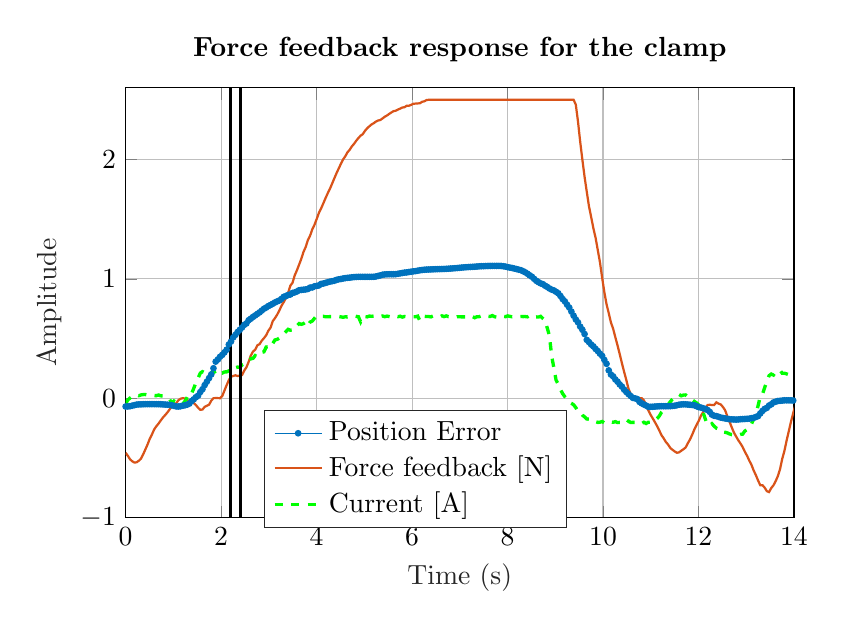
\begin{tikzpicture}

\begin{axis}[%
width=0.7\columnwidth,
height=0.45\columnwidth,
at={(2.512in,1.147in)},
scale only axis,
xmin=0,
xmax=14,
xlabel style={font=\color{white!15!black}},
xlabel={Time (s)},
ymin=-1,
ymax=2.6,
ylabel style={font=\color{white!15!black}},
ylabel={Amplitude},
axis background/.style={fill=white},
title style={font=\bfseries},
title={Force feedback response for the clamp},
xmajorgrids,
ymajorgrids,
legend style={legend cell align=left, align=left, draw=white!15!black, at={(0.66,0.25)}}
]

\addplot [color=mycolor1, draw=none, mark=*, mark size=1,mark options={solid, mycolor1}]
  table[row sep=crcr]{%
0	-0.069839\\
0.046	-0.0691929999999998\\
0.092	-0.0674169999999998\\
0.138	-0.0627580000000001\\
0.184	-0.0585599999999999\\
0.23	-0.053715\\
0.276	-0.052262\\
0.322	-0.0517779999999999\\
0.368	-0.0508089999999999\\
0.414	-0.050325\\
0.46	-0.0500019999999999\\
0.506	-0.0500019999999999\\
0.552	-0.0500019999999999\\
0.598	-0.0500019999999999\\
0.644	-0.050233\\
0.69	-0.0504629999999999\\
0.736	-0.0509360000000001\\
0.782	-0.0523979999999999\\
0.828	-0.0533170000000001\\
0.874	-0.0544640000000001\\
0.92	-0.0558380000000001\\
0.966	-0.059431\\
1.012	-0.0646089999999999\\
1.058	-0.069102\\
1.104	-0.070166\\
1.15	-0.0678619999999999\\
1.196	-0.0632820000000001\\
1.242	-0.0596559999999999\\
1.288	-0.054314\\
1.334	-0.045984\\
1.38	-0.0253700000000001\\
1.426	-0.00976399999999988\\
1.472	0.00805999999999996\\
1.518	0.0212249999999999\\
1.564	0.051482\\
1.61	0.0750869999999999\\
1.656	0.109672\\
1.702	0.138343\\
1.748	0.168177\\
1.794	0.199188\\
1.84	0.250473\\
1.886	0.306211\\
1.932	0.324103\\
1.978	0.347052\\
2.024	0.362787\\
2.07	0.383776\\
2.116	0.406007\\
2.162	0.449559\\
2.208	0.474824\\
2.254	0.508958\\
2.3	0.530804\\
2.346	0.554437\\
2.392	0.572537\\
2.438	0.591942\\
2.484	0.614258\\
2.53	0.625926\\
2.576	0.652916\\
2.622	0.665954\\
2.668	0.680707\\
2.714	0.6931054\\
2.76	0.7064931\\
2.806	0.7187228\\
2.852	0.7341136\\
2.898	0.7492224\\
2.944	0.7593239\\
2.99	0.7720971\\
3.036	0.7809118\\
3.082	0.7910974\\
3.128	0.8020223\\
3.174	0.81066\\
3.22	0.8186307\\
3.266	0.8319814\\
3.312	0.8492741\\
3.358	0.8558223\\
3.404	0.8646376\\
3.45	0.868742\\
3.496	0.8814436\\
3.542	0.8863328\\
3.588	0.8938385\\
3.634	0.9044656\\
3.68	0.9069801\\
3.726	0.9089659\\
3.772	0.9109976\\
3.818	0.9148639\\
3.864	0.9265554\\
3.91	0.9278963\\
3.956	0.9373217\\
4.002	0.940841\\
4.048	0.9445568\\
4.094	0.95726415\\
4.14	0.9604788\\
4.186	0.96597617\\
4.232	0.97119919\\
4.278	0.97641396\\
4.324	0.9801821\\
4.37	0.9838232\\
4.416	0.9907857\\
4.462	0.99572\\
4.508	0.9983443\\
4.554	1.0027004\\
4.6	1.0057562\\
4.646	1.0081051\\
4.692	1.0098843\\
4.738	1.0125273\\
4.784	1.0145615\\
4.83	1.015724\\
4.876	1.0164667\\
4.922	1.0164667\\
4.968	1.0164667\\
5.014	1.0164667\\
5.06	1.0164667\\
5.106	1.0164667\\
5.152	1.0164667\\
5.198	1.017048\\
5.244	1.0196638\\
5.29	1.0246052\\
5.336	1.0286748\\
5.382	1.0344887\\
5.428	1.0368141\\
5.474	1.0379768\\
5.52	1.0385582\\
5.566	1.0385582\\
5.612	1.0385582\\
5.658	1.0391396\\
5.704	1.0420462\\
5.75	1.045534\\
5.796	1.0490214\\
5.842	1.0522178\\
5.888	1.0536705\\
5.934	1.0571568\\
5.98	1.059633\\
6.026	1.062445\\
6.072	1.0644935\\
6.118	1.0679936\\
6.164	1.0718006\\
6.21	1.0739226\\
6.256	1.0760766\\
6.302	1.0773746\\
6.348	1.0781606\\
6.394	1.0786866\\
6.44	1.0796386\\
6.486	1.0806226\\
6.532	1.0811326\\
6.578	1.0815816\\
6.624	1.0821676\\
6.67	1.0826356\\
6.716	1.0836156\\
6.762	1.0849286\\
6.808	1.0862066\\
6.854	1.0874876\\
6.9	1.0889816\\
6.946	1.0904386\\
6.992	1.0921886\\
7.038	1.0943516\\
7.084	1.0958206\\
7.13	1.0971756\\
7.176	1.0983656\\
7.222	1.0995076\\
7.268	1.1005966\\
7.314	1.1015086\\
7.36	1.1031166\\
7.406	1.1045566\\
7.452	1.1057716\\
7.498	1.1059546\\
7.544	1.1072416\\
7.59	1.1076566\\
7.636	1.1080086\\
7.682	1.1083606\\
7.728	1.1083606\\
7.774	1.1082496\\
7.82	1.1082496\\
7.866	1.1078506\\
7.912	1.1055066\\
7.958	1.1023436\\
8.004	1.0977176\\
8.05	1.0940366\\
8.096	1.0909596\\
8.142	1.0861036\\
8.188	1.0816106\\
8.234	1.0766646\\
8.28	1.0723386\\
8.326	1.0637863\\
8.372	1.0543818\\
8.418	1.0428257\\
8.464	1.029448\\
8.51	1.0175659\\
8.556	1.0002029\\
8.602	0.9837055\\
8.648	0.97187785\\
8.694	0.96156563\\
8.74	0.9554396\\
8.786	0.942303\\
8.832	0.9318928\\
8.878	0.9191614\\
8.924	0.9095359\\
8.97	0.9029574\\
9.016	0.8912888\\
9.062	0.879097\\
9.108	0.8563865\\
9.154	0.8307516\\
9.2	0.8113894\\
9.246	0.7837317\\
9.292	0.7592755\\
9.338	0.725409\\
9.384	0.691096\\
9.43	0.659743\\
9.476	0.635184\\
9.522	0.599631\\
9.568	0.572746\\
9.614	0.537474\\
9.66	0.488529\\
9.706	0.470013\\
9.752	0.449131\\
9.798	0.434072\\
9.844	0.412879\\
9.89	0.394881\\
9.936	0.372667\\
9.982	0.354272\\
10.028	0.320757\\
10.074	0.287993\\
10.12	0.232964\\
10.166	0.197741\\
10.212	0.18275\\
10.258	0.156795\\
10.304	0.138484\\
10.35	0.114872\\
10.396	0.097008\\
10.442	0.071595\\
10.488	0.05155\\
10.534	0.034095\\
10.58	0.0179400000000001\\
10.626	0.002305\\
10.672	-0.00167099999999998\\
10.718	-0.00769699999999984\\
10.764	-0.030978\\
10.81	-0.0429710000000001\\
10.856	-0.053148\\
10.902	-0.0618189999999998\\
10.948	-0.0720810000000001\\
10.994	-0.0724389999999999\\
11.04	-0.0717700000000001\\
11.086	-0.0703040000000001\\
11.132	-0.068948\\
11.178	-0.0678830000000001\\
11.224	-0.067339\\
11.27	-0.067339\\
11.316	-0.067339\\
11.362	-0.0671580000000001\\
11.408	-0.0669960000000001\\
11.454	-0.065239\\
11.5	-0.063358\\
11.546	-0.0595410000000001\\
11.592	-0.054964\\
11.638	-0.052603\\
11.684	-0.051604\\
11.73	-0.0518610000000002\\
11.776	-0.053331\\
11.822	-0.0551919999999999\\
11.868	-0.0570810000000002\\
11.914	-0.059763\\
11.96	-0.0673490000000001\\
12.006	-0.075137\\
12.052	-0.0787260000000001\\
12.098	-0.084632\\
12.144	-0.090457\\
12.19	-0.099099\\
12.236	-0.115104\\
12.282	-0.138322\\
12.328	-0.147654\\
12.374	-0.150269\\
12.42	-0.156016\\
12.466	-0.1626\\
12.512	-0.166108\\
12.558	-0.169979\\
12.604	-0.172681\\
12.65	-0.176454\\
12.696	-0.177723\\
12.742	-0.178345\\
12.788	-0.179376\\
12.834	-0.178237\\
12.88	-0.176378\\
12.926	-0.175254\\
12.972	-0.174123\\
13.018	-0.172999\\
13.064	-0.171682\\
13.11	-0.167706\\
13.156	-0.164679\\
13.202	-0.157745\\
13.248	-0.1501\\
13.294	-0.127712\\
13.34	-0.106903\\
13.386	-0.0901689999999999\\
13.432	-0.0812360000000001\\
13.478	-0.0620539999999998\\
13.524	-0.0516510000000001\\
13.57	-0.035822\\
13.616	-0.029779\\
13.662	-0.0236429999999999\\
13.708	-0.0221900000000002\\
13.754	-0.0202520000000002\\
13.8	-0.0181120000000001\\
13.846	-0.018038\\
13.892	-0.018243\\
13.938	-0.0184470000000001\\
13.984	-0.019682\\
14.03	-0.0207010000000001\\
14.076	-0.0221230000000001\\
14.122	-0.023096\\
14.168	-0.023096\\
14.214	-0.023096\\
14.26	-0.0234529999999999\\
14.306	-0.024132\\
14.352	-0.0254239999999999\\
14.398	-0.0299449999999999\\
14.444	-0.033693\\
14.49	-0.0363100000000001\\
14.536	-0.0374399999999999\\
14.582	-0.0393779999999999\\
14.628	-0.039701\\
14.674	-0.0398689999999999\\
14.72	-0.0398770000000002\\
14.766	-0.039682\\
14.812	-0.039682\\
14.858	-0.039682\\
14.904	-0.039682\\
14.95	-0.039682\\
14.996	-0.0391299999999999\\
15.042	-0.0387390000000001\\
15.088	-0.0385439999999999\\
15.134	-0.038152\\
15.18	-0.0377609999999999\\
15.226	-0.0377609999999999\\
15.272	-0.0377609999999999\\
15.318	-0.0377609999999999\\
15.364	-0.0377609999999999\\
15.41	-0.0377609999999999\\
15.456	-0.0375649999999998\\
15.502	-0.0375649999999998\\
15.548	-0.036365\\
15.594	-0.0331220000000001\\
15.64	-0.030756\\
15.686	-0.0297510000000001\\
15.732	-0.02959\\
15.778	-0.028459\\
};
\addlegendentry{Position Error}

\addplot [color=mycolor2, thick]
  table[row sep=crcr]{%
0	-0.457965\\
0.046	-0.482939\\
0.092	-0.512125\\
0.138	-0.528618\\
0.184	-0.539522\\
0.23	-0.537151\\
0.276	-0.524402\\
0.322	-0.507127\\
0.368	-0.470289\\
0.414	-0.428809\\
0.46	-0.387254\\
0.506	-0.339716\\
0.552	-0.303282\\
0.598	-0.26139\\
0.644	-0.235044\\
0.69	-0.212801\\
0.736	-0.186553\\
0.782	-0.161903\\
0.828	-0.14172\\
0.874	-0.120005\\
0.92	-0.094566\\
0.966	-0.0684803\\
1.012	-0.0608241\\
1.058	-0.0433587\\
1.104	-0.0174891\\
1.15	-0.00521286\\
1.196	0.000178016\\
1.242	-0.00297375\\
1.288	-0.0138918\\
1.334	-0.026421\\
1.38	-0.0261145\\
1.426	-0.0405375\\
1.472	-0.0576523\\
1.518	-0.0799315\\
1.564	-0.0976721\\
1.61	-0.0951568\\
1.656	-0.0724242\\
1.702	-0.0633538\\
1.748	-0.0541451\\
1.794	-0.021039\\
1.84	0.000387498\\
1.886	0.00063466\\
1.932	0.000510842\\
1.978	1.40871e-05\\
2.024	0.0176141\\
2.07	0.0641683\\
2.116	0.109299\\
2.162	0.152024\\
2.208	0.179542\\
2.254	0.185892\\
2.3	0.191742\\
2.346	0.185386\\
2.392	0.189675\\
2.438	0.193986\\
2.484	0.230854\\
2.53	0.257935\\
2.576	0.303503\\
2.622	0.357063\\
2.668	0.390772\\
2.714	0.405952\\
2.76	0.443154\\
2.806	0.452801\\
2.852	0.481958\\
2.898	0.503039\\
2.944	0.527297\\
2.99	0.56528\\
3.036	0.591189\\
3.082	0.645425\\
3.128	0.670379\\
3.174	0.699748\\
3.22	0.735109\\
3.266	0.774628\\
3.312	0.805072\\
3.358	0.83938\\
3.404	0.882872\\
3.45	0.942162\\
3.496	0.967106\\
3.542	1.02907\\
3.588	1.07135\\
3.634	1.11914\\
3.68	1.16782\\
3.726	1.22586\\
3.772	1.26648\\
3.818	1.32544\\
3.864	1.36167\\
3.91	1.41453\\
3.956	1.45284\\
4.002	1.50118\\
4.048	1.55186\\
4.094	1.58921\\
4.14	1.63147\\
4.186	1.67488\\
4.232	1.71576\\
4.278	1.75288\\
4.324	1.79633\\
4.37	1.84079\\
4.416	1.88369\\
4.462	1.92324\\
4.508	1.96243\\
4.554	1.99936\\
4.6	2.02567\\
4.646	2.05945\\
4.692	2.08038\\
4.738	2.10928\\
4.784	2.13069\\
4.83	2.15696\\
4.876	2.17937\\
4.922	2.19947\\
4.968	2.21219\\
5.014	2.24018\\
5.06	2.26189\\
5.106	2.27821\\
5.152	2.29389\\
5.198	2.3042\\
5.244	2.31804\\
5.29	2.32692\\
5.336	2.33094\\
5.382	2.34414\\
5.428	2.35817\\
5.474	2.36845\\
5.52	2.38155\\
5.566	2.39363\\
5.612	2.40496\\
5.658	2.40824\\
5.704	2.41806\\
5.75	2.42631\\
5.796	2.4351\\
5.842	2.43808\\
5.888	2.45076\\
5.934	2.45048\\
5.98	2.45716\\
6.026	2.4668\\
6.072	2.46822\\
6.118	2.46973\\
6.164	2.47081\\
6.21	2.48353\\
6.256	2.48696\\
6.302	2.49787\\
6.348	2.5\\
6.394	2.5\\
6.44	2.5\\
6.486	2.5\\
6.532	2.49992\\
6.578	2.5\\
6.624	2.5\\
6.67	2.5\\
6.716	2.5\\
6.762	2.5\\
6.808	2.5\\
6.854	2.5\\
6.9	2.5\\
6.946	2.5\\
6.992	2.5\\
7.038	2.5\\
7.084	2.5\\
7.13	2.5\\
7.176	2.5\\
7.222	2.5\\
7.268	2.5\\
7.314	2.5\\
7.36	2.5\\
7.406	2.5\\
7.452	2.5\\
7.498	2.5\\
7.544	2.5\\
7.59	2.5\\
7.636	2.5\\
7.682	2.5\\
7.728	2.5\\
7.774	2.5\\
7.82	2.5\\
7.866	2.5\\
7.912	2.5\\
7.958	2.5\\
8.004	2.5\\
8.05	2.5\\
8.096	2.5\\
8.142	2.5\\
8.188	2.5\\
8.234	2.5\\
8.28	2.5\\
8.326	2.5\\
8.372	2.5\\
8.418	2.5\\
8.464	2.5\\
8.51	2.5\\
8.556	2.5\\
8.602	2.5\\
8.648	2.5\\
8.694	2.5\\
8.74	2.5\\
8.786	2.5\\
8.832	2.5\\
8.878	2.5\\
8.924	2.5\\
8.97	2.5\\
9.016	2.5\\
9.062	2.5\\
9.108	2.5\\
9.154	2.5\\
9.2	2.5\\
9.246	2.5\\
9.292	2.5\\
9.338	2.5\\
9.384	2.5\\
9.43	2.45972\\
9.476	2.31758\\
9.522	2.14825\\
9.568	1.99722\\
9.614	1.85379\\
9.66	1.72876\\
9.706	1.60717\\
9.752	1.51777\\
9.798	1.42349\\
9.844	1.34486\\
9.89	1.24209\\
9.936	1.13853\\
9.982	1.0087\\
10.028	0.888403\\
10.074	0.786921\\
10.12	0.712798\\
10.166	0.633521\\
10.212	0.58201\\
10.258	0.510575\\
10.304	0.442393\\
10.35	0.369444\\
10.396	0.293081\\
10.442	0.220909\\
10.488	0.152474\\
10.534	0.078849\\
10.58	0.0342911\\
10.626	0.000124028\\
10.672	0.000301921\\
10.718	0.000252726\\
10.764	0.000330059\\
10.81	0.000273753\\
10.856	-0.0174561\\
10.902	-0.0569983\\
10.948	-0.101156\\
10.994	-0.137496\\
11.04	-0.16853\\
11.086	-0.20015\\
11.132	-0.233028\\
11.178	-0.269616\\
11.224	-0.309738\\
11.27	-0.335806\\
11.316	-0.366884\\
11.362	-0.387696\\
11.408	-0.416516\\
11.454	-0.432208\\
11.5	-0.445834\\
11.546	-0.45736\\
11.592	-0.45423\\
11.638	-0.440815\\
11.684	-0.428176\\
11.73	-0.413655\\
11.776	-0.377847\\
11.822	-0.346186\\
11.868	-0.30626\\
11.914	-0.261468\\
11.96	-0.224553\\
12.006	-0.188972\\
12.052	-0.146403\\
12.098	-0.116957\\
12.144	-0.0867584\\
12.19	-0.0573152\\
12.236	-0.0552171\\
12.282	-0.0574377\\
12.328	-0.0575676\\
12.374	-0.0349744\\
12.42	-0.046042\\
12.466	-0.0523814\\
12.512	-0.0740595\\
12.558	-0.101582\\
12.604	-0.151553\\
12.65	-0.197503\\
12.696	-0.243833\\
12.742	-0.288091\\
12.788	-0.321104\\
12.834	-0.352334\\
12.88	-0.379869\\
12.926	-0.410188\\
12.972	-0.449443\\
13.018	-0.483054\\
13.064	-0.523156\\
13.11	-0.558781\\
13.156	-0.606164\\
13.202	-0.644778\\
13.248	-0.689715\\
13.294	-0.72931\\
13.34	-0.729152\\
13.386	-0.749485\\
13.432	-0.779093\\
13.478	-0.786947\\
13.524	-0.753038\\
13.57	-0.730523\\
13.616	-0.695568\\
13.662	-0.65353\\
13.708	-0.595233\\
13.754	-0.50868\\
13.8	-0.441981\\
13.846	-0.355192\\
13.892	-0.275813\\
13.938	-0.196536\\
13.984	-0.125382\\
14.03	-0.0564939\\
14.076	0.000372308\\
14.122	0.000553329\\
14.168	0.000643569\\
14.214	0.000462548\\
14.26	0.00539057\\
14.306	0.0388688\\
14.352	0.0787901\\
14.398	0.106753\\
14.444	0.130374\\
14.49	0.152278\\
14.536	0.170294\\
14.582	0.159808\\
14.628	0.155049\\
14.674	0.143513\\
14.72	0.12149\\
14.766	0.0911616\\
14.812	0.0673271\\
14.858	0.0494943\\
14.904	0.0241393\\
14.95	0.00996927\\
14.996	0.000383604\\
15.042	1.06228e-05\\
15.088	0.000199578\\
15.134	0.00057731\\
15.18	0.000486604\\
15.226	0.000296169\\
15.272	0.000202064\\
15.318	0.000297389\\
15.364	0.000202064\\
15.41	0.000297389\\
15.456	0.000682615\\
15.502	0.000490612\\
15.548	0.000398122\\
15.594	0.00049462\\
15.64	0.000399735\\
15.686	0.000596488\\
15.732	0.000108347\\
15.778	0.000401348\\
};
\addlegendentry{Force feedback [N]}

\addplot [color=green, dashed, very thick]
  table[row sep=crcr]{%
0	-0.0462933\\
0.046	-0.0146618\\
0.092	0.00131416\\
0.138	0.0156918\\
0.184	0.0268745\\
0.23	0.0278339\\
0.276	0.0204849\\
0.322	0.027195\\
0.368	0.0300694\\
0.414	0.0303898\\
0.46	0.026556\\
0.506	0.0262356\\
0.552	0.0275135\\
0.598	0.0217628\\
0.644	0.0211239\\
0.69	0.026556\\
0.736	0.0195255\\
0.782	0.0188866\\
0.828	0.0115376\\
0.874	-0.00220108\\
0.92	-0.00891113\\
0.966	-0.0418205\\
1.012	-0.0236073\\
1.058	-0.0344715\\
1.104	-0.0450153\\
1.15	-0.0504456\\
1.196	-0.0485287\\
1.242	-0.0261631\\
1.288	0.0057869\\
1.334	0.0434895\\
1.38	0.0380573\\
1.426	0.081192\\
1.472	0.129118\\
1.518	0.168417\\
1.564	0.209953\\
1.61	0.222414\\
1.656	0.213787\\
1.702	0.216024\\
1.748	0.229124\\
1.794	0.210911\\
1.84	0.235514\\
1.886	0.200048\\
1.932	0.214746\\
1.978	0.216024\\
2.024	0.209953\\
2.07	0.219858\\
2.116	0.220497\\
2.162	0.229124\\
2.208	0.231041\\
2.254	0.261074\\
2.3	0.255003\\
2.346	0.260756\\
2.392	0.25724\\
2.438	0.278328\\
2.484	0.286955\\
2.53	0.301332\\
2.576	0.316988\\
2.622	0.329769\\
2.668	0.333603\\
2.714	0.356928\\
2.76	0.346703\\
2.806	0.368429\\
2.852	0.383766\\
2.898	0.388559\\
2.944	0.428497\\
2.99	0.431053\\
3.036	0.468117\\
3.082	0.458851\\
3.128	0.487926\\
3.174	0.492718\\
3.22	0.502623\\
3.266	0.524349\\
3.312	0.540007\\
3.358	0.557259\\
3.404	0.57675\\
3.45	0.56908\\
3.496	0.571957\\
3.542	0.575151\\
3.588	0.605825\\
3.634	0.625315\\
3.68	0.618925\\
3.726	0.624355\\
3.772	0.636816\\
3.818	0.607422\\
3.864	0.637775\\
3.91	0.646082\\
3.956	0.668768\\
4.002	0.687618\\
4.048	0.682827\\
4.094	0.686979\\
4.14	0.686022\\
4.186	0.682186\\
4.232	0.681547\\
4.278	0.683466\\
4.324	0.682507\\
4.37	0.681868\\
4.416	0.682827\\
4.462	0.684423\\
4.508	0.681547\\
4.554	0.677713\\
4.6	0.681868\\
4.646	0.680908\\
4.692	0.685062\\
4.738	0.685383\\
4.784	0.690174\\
4.83	0.685383\\
4.876	0.682507\\
4.922	0.640331\\
4.968	0.684105\\
5.014	0.683466\\
5.06	0.681229\\
5.106	0.687939\\
5.152	0.685701\\
5.198	0.688257\\
5.244	0.681229\\
5.29	0.679312\\
5.336	0.684744\\
5.382	0.688896\\
5.428	0.682827\\
5.474	0.687618\\
5.52	0.684105\\
5.566	0.67963\\
5.612	0.678034\\
5.658	0.687939\\
5.704	0.682507\\
5.75	0.686661\\
5.796	0.678991\\
5.842	0.684744\\
5.888	0.681868\\
5.934	0.685701\\
5.98	0.687939\\
6.026	0.681868\\
6.072	0.681868\\
6.118	0.687618\\
6.164	0.648638\\
6.21	0.681229\\
6.256	0.685701\\
6.302	0.684423\\
6.348	0.683784\\
6.394	0.681229\\
6.44	0.688578\\
6.486	0.681868\\
6.532	0.682186\\
6.578	0.68059\\
6.624	0.689856\\
6.67	0.683466\\
6.716	0.689856\\
6.762	0.682827\\
6.808	0.681229\\
6.854	0.680908\\
6.9	0.676756\\
6.946	0.682507\\
6.992	0.682827\\
7.038	0.680908\\
7.084	0.681229\\
7.13	0.68059\\
7.176	0.687939\\
7.222	0.678352\\
7.268	0.682827\\
7.314	0.6742\\
7.36	0.682827\\
7.406	0.682827\\
7.452	0.690174\\
7.498	0.681547\\
7.544	0.686979\\
7.59	0.685383\\
7.636	0.684744\\
7.682	0.692091\\
7.728	0.682186\\
7.774	0.678673\\
7.82	0.684744\\
7.866	0.692091\\
7.912	0.685383\\
7.958	0.682827\\
8.004	0.689535\\
8.05	0.685383\\
8.096	0.681547\\
8.142	0.683146\\
8.188	0.679951\\
8.234	0.682186\\
8.28	0.683784\\
8.326	0.683466\\
8.372	0.683784\\
8.418	0.681547\\
8.464	0.69273\\
8.51	0.680269\\
8.556	0.678034\\
8.602	0.680908\\
8.648	0.67963\\
8.694	0.685701\\
8.74	0.667809\\
8.786	0.65439\\
8.832	0.587612\\
8.878	0.522753\\
8.924	0.353092\\
8.97	0.255323\\
9.016	0.151484\\
9.062	0.117296\\
9.108	0.0735226\\
9.154	0.0380573\\
9.2	0.0124969\\
9.246	-0.00699234\\
9.292	-0.0335121\\
9.338	-0.043417\\
9.384	-0.0552387\\
9.43	-0.0792027\\
9.476	-0.110834\\
9.522	-0.115625\\
9.568	-0.141827\\
9.614	-0.156843\\
9.66	-0.174736\\
9.706	-0.176014\\
9.752	-0.183681\\
9.798	-0.182404\\
9.844	-0.197102\\
9.89	-0.203171\\
9.936	-0.201254\\
9.982	-0.195503\\
10.028	-0.207645\\
10.074	-0.211479\\
10.12	-0.208923\\
10.166	-0.199337\\
10.212	-0.202213\\
10.258	-0.196781\\
10.304	-0.204449\\
10.35	-0.202852\\
10.396	-0.202213\\
10.442	-0.209881\\
10.488	-0.214354\\
10.534	-0.191988\\
10.58	-0.20381\\
10.626	-0.202532\\
10.672	-0.203171\\
10.718	-0.208284\\
10.764	-0.21755\\
10.81	-0.212437\\
10.856	-0.201574\\
10.902	-0.212118\\
10.948	-0.202532\\
10.994	-0.201893\\
11.04	-0.190392\\
11.086	-0.184641\\
11.132	-0.171221\\
11.178	-0.150454\\
11.224	-0.119141\\
11.27	-0.100929\\
11.316	-0.0760078\\
11.362	-0.0552387\\
11.408	-0.0299988\\
11.454	-0.0085907\\
11.5	0.00866318\\
11.546	0.0224018\\
11.592	0.0313473\\
11.638	0.019846\\
11.684	0.0259171\\
11.73	0.027195\\
11.776	0.011219\\
11.822	0.00866318\\
11.868	-0.0140228\\
11.914	-0.0271225\\
11.96	-0.0399017\\
12.006	-0.058115\\
12.052	-0.0986919\\
12.098	-0.1201\\
12.144	-0.177292\\
12.19	-0.223619\\
12.236	-0.228094\\
12.282	-0.213715\\
12.328	-0.234484\\
12.374	-0.251417\\
12.42	-0.258127\\
12.466	-0.280811\\
12.512	-0.283369\\
12.558	-0.285925\\
12.604	-0.290716\\
12.65	-0.299664\\
12.696	-0.305414\\
12.742	-0.307331\\
12.788	-0.305414\\
12.834	-0.309568\\
12.88	-0.303177\\
12.926	-0.30126\\
12.972	-0.274742\\
13.018	-0.263878\\
13.064	-0.237679\\
13.11	-0.216272\\
13.156	-0.174736\\
13.202	-0.137352\\
13.248	-0.0641861\\
13.294	0.0150528\\
13.34	0.0339031\\
13.386	0.0882206\\
13.432	0.139662\\
13.478	0.188227\\
13.524	0.202286\\
13.57	0.193338\\
13.616	0.21826\\
13.662	0.226248\\
13.708	0.234556\\
13.754	0.208355\\
13.8	0.208994\\
13.846	0.203243\\
13.892	0.196533\\
13.938	0.189505\\
13.984	0.18631\\
14.03	0.17321\\
14.076	0.157873\\
14.122	0.146051\\
14.168	0.111225\\
14.214	0.0952492\\
14.26	0.0613823\\
14.306	0.0450859\\
14.352	0.0188866\\
14.398	-0.00571442\\
14.444	-0.0213718\\
14.49	-0.0296783\\
14.536	-0.0402222\\
14.582	-0.0309563\\
14.628	-0.0306377\\
14.674	-0.036068\\
14.72	-0.0379848\\
14.766	-0.0357494\\
14.812	-0.0312767\\
14.858	-0.0383053\\
14.904	-0.0303173\\
14.95	-0.0306377\\
14.996	-0.0296783\\
15.042	-0.0216904\\
15.088	-0.0216904\\
15.134	-0.0137024\\
15.18	0.000675201\\
15.226	-0.00251961\\
15.272	0.0124969\\
15.318	0.0131359\\
15.364	0.0211239\\
15.41	0.0255966\\
15.456	0.0287914\\
15.502	0.0310287\\
15.548	0.0326252\\
15.594	0.0262356\\
15.64	0.0294304\\
15.686	0.0422115\\
15.732	0.0479622\\
15.778	0.0447674\\
};
\addlegendentry{Current [A]}
\addplot [color=black, forget plot, very thick]
  table[row sep=crcr]{%
2.4	-1\\
2.4 2.6\\
};\addplot [color=black, forget plot, very thick]
  table[row sep=crcr]{%
2.2	-1\\
2.2	2.6\\
};
\end{axis}
\end{tikzpicture}%
\end{figure}
\end{frame}

\begin{frame}<beamer>
\vspace*{1.5cm}
\begin{figure}[h]
\centering
	\begin{tikzpicture}
	%axes
	\draw [->,thick] (-3,0) -- (3,0);
	\draw [->,thick] (0,-2.2) -- (0,2.2);
	%model
	\draw [ultra thick, color=blue] (0,-1.6) -- (0,1.6);
	\draw [ultra thick, color=blue] (0,1.6) -- (3,1.6);
	\draw [ultra thick, color=blue] (0,-1.6) -- (-3,-1.6);
	%name of axis and variables
	\node at (-0.4,1.6) {$\tau_s$};
	\draw (-0.22,1.6) -- (-0.1,1.6);

	\node at (3,0.4) {$\omega$};
	\node at (0.4,2.2) {$\tau_f$};

	\end{tikzpicture}
\caption{Static and Coulomb friction model}
\label{fig:new_friction_model}
\end{figure}
\end{frame}


\begin{frame}<beamer>
\vspace*{1.5cm}
\begin{figure}
\centering
% This file was created by matlab2tikz.
%
%The latest updates can be retrieved from
%  http://www.mathworks.com/matlabcentral/fileexchange/22022-matlab2tikz-matlab2tikz
%where you can also make suggestions and rate matlab2tikz.
%
\definecolor{mycolor1}{rgb}{0.00000,0.44700,0.74100}%
\definecolor{mycolor2}{rgb}{0.85000,0.32500,0.09800}%
%
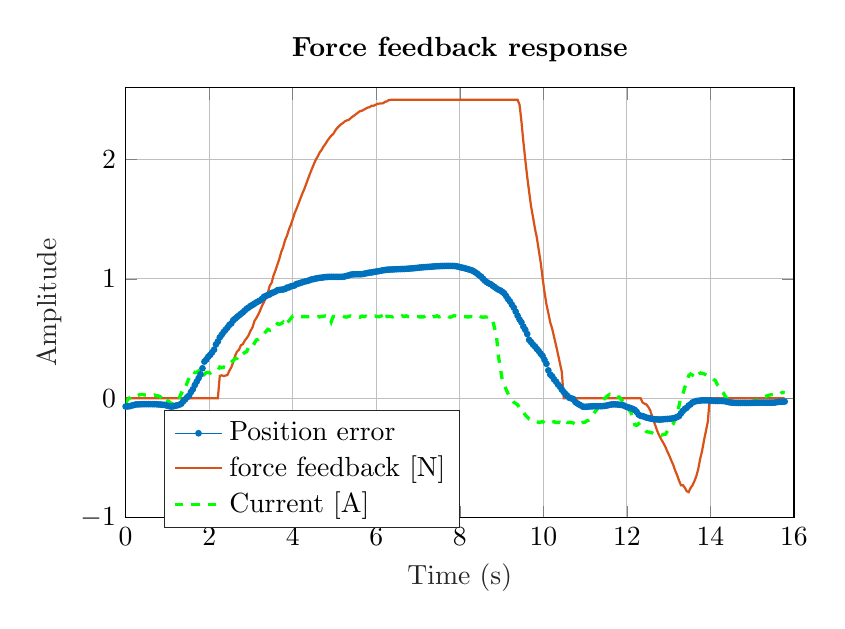
\begin{tikzpicture}

\begin{axis}[%
width=0.7\columnwidth,
height=0.45\columnwidth,
at={(2.512in,1.147in)},
scale only axis,
xmin=0,
xmax=16,
xlabel style={font=\color{white!15!black}},
xlabel={Time (s)},
ymin=-1,
ymax=2.6,
ylabel style={font=\color{white!15!black}},
ylabel={Amplitude},
axis background/.style={fill=white},
title style={font=\bfseries},
title={Force feedback response},
xmajorgrids,
ymajorgrids,
legend style={legend cell align=left, align=left, draw=white!15!black,  at={(0.5,0.25)}}
]
\addplot [color=mycolor1, draw=none, mark=*,mark size= 1, mark options={,solid, mycolor1}]
  table[row sep=crcr]{%
0	-0.069839\\
0.046	-0.0691929999999998\\
0.092	-0.0674169999999998\\
0.138	-0.0627580000000001\\
0.184	-0.0585599999999999\\
0.23	-0.053715\\
0.276	-0.052262\\
0.322	-0.0517779999999999\\
0.368	-0.0508089999999999\\
0.414	-0.050325\\
0.46	-0.0500019999999999\\
0.506	-0.0500019999999999\\
0.552	-0.0500019999999999\\
0.598	-0.0500019999999999\\
0.644	-0.050233\\
0.69	-0.0504629999999999\\
0.736	-0.0509360000000001\\
0.782	-0.0523979999999999\\
0.828	-0.0533170000000001\\
0.874	-0.0544640000000001\\
0.92	-0.0558380000000001\\
0.966	-0.059431\\
1.012	-0.0646089999999999\\
1.058	-0.069102\\
1.104	-0.070166\\
1.15	-0.0678619999999999\\
1.196	-0.0632820000000001\\
1.242	-0.0596559999999999\\
1.288	-0.054314\\
1.334	-0.045984\\
1.38	-0.0253700000000001\\
1.426	-0.00976399999999988\\
1.472	0.00805999999999996\\
1.518	0.0212249999999999\\
1.564	0.051482\\
1.61	0.0750869999999999\\
1.656	0.109672\\
1.702	0.138343\\
1.748	0.168177\\
1.794	0.199188\\
1.84	0.250473\\
1.886	0.306211\\
1.932	0.324103\\
1.978	0.347052\\
2.024	0.362787\\
2.07	0.383776\\
2.116	0.406007\\
2.162	0.449559\\
2.208	0.474824\\
2.254	0.508958\\
2.3	0.530804\\
2.346	0.554437\\
2.392	0.572537\\
2.438	0.591942\\
2.484	0.614258\\
2.53	0.625926\\
2.576	0.652916\\
2.622	0.665954\\
2.668	0.680707\\
2.714	0.6931054\\
2.76	0.7064931\\
2.806	0.7187228\\
2.852	0.7341136\\
2.898	0.7492224\\
2.944	0.7593239\\
2.99	0.7720971\\
3.036	0.7809118\\
3.082	0.7910974\\
3.128	0.8020223\\
3.174	0.81066\\
3.22	0.8186307\\
3.266	0.8319814\\
3.312	0.8492741\\
3.358	0.8558223\\
3.404	0.8646376\\
3.45	0.868742\\
3.496	0.8814436\\
3.542	0.8863328\\
3.588	0.8938385\\
3.634	0.9044656\\
3.68	0.9069801\\
3.726	0.9089659\\
3.772	0.9109976\\
3.818	0.9148639\\
3.864	0.9265554\\
3.91	0.9278963\\
3.956	0.9373217\\
4.002	0.940841\\
4.048	0.9445568\\
4.094	0.95726415\\
4.14	0.9604788\\
4.186	0.96597617\\
4.232	0.97119919\\
4.278	0.97641396\\
4.324	0.9801821\\
4.37	0.9838232\\
4.416	0.9907857\\
4.462	0.99572\\
4.508	0.9983443\\
4.554	1.0027004\\
4.6	1.0057562\\
4.646	1.0081051\\
4.692	1.0098843\\
4.738	1.0125273\\
4.784	1.0145615\\
4.83	1.015724\\
4.876	1.0164667\\
4.922	1.0164667\\
4.968	1.0164667\\
5.014	1.0164667\\
5.06	1.0164667\\
5.106	1.0164667\\
5.152	1.0164667\\
5.198	1.017048\\
5.244	1.0196638\\
5.29	1.0246052\\
5.336	1.0286748\\
5.382	1.0344887\\
5.428	1.0368141\\
5.474	1.0379768\\
5.52	1.0385582\\
5.566	1.0385582\\
5.612	1.0385582\\
5.658	1.0391396\\
5.704	1.0420462\\
5.75	1.045534\\
5.796	1.0490214\\
5.842	1.0522178\\
5.888	1.0536705\\
5.934	1.0571568\\
5.98	1.059633\\
6.026	1.062445\\
6.072	1.0644935\\
6.118	1.0679936\\
6.164	1.0718006\\
6.21	1.0739226\\
6.256	1.0760766\\
6.302	1.0773746\\
6.348	1.0781606\\
6.394	1.0786866\\
6.44	1.0796386\\
6.486	1.0806226\\
6.532	1.0811326\\
6.578	1.0815816\\
6.624	1.0821676\\
6.67	1.0826356\\
6.716	1.0836156\\
6.762	1.0849286\\
6.808	1.0862066\\
6.854	1.0874876\\
6.9	1.0889816\\
6.946	1.0904386\\
6.992	1.0921886\\
7.038	1.0943516\\
7.084	1.0958206\\
7.13	1.0971756\\
7.176	1.0983656\\
7.222	1.0995076\\
7.268	1.1005966\\
7.314	1.1015086\\
7.36	1.1031166\\
7.406	1.1045566\\
7.452	1.1057716\\
7.498	1.1059546\\
7.544	1.1072416\\
7.59	1.1076566\\
7.636	1.1080086\\
7.682	1.1083606\\
7.728	1.1083606\\
7.774	1.1082496\\
7.82	1.1082496\\
7.866	1.1078506\\
7.912	1.1055066\\
7.958	1.1023436\\
8.004	1.0977176\\
8.05	1.0940366\\
8.096	1.0909596\\
8.142	1.0861036\\
8.188	1.0816106\\
8.234	1.0766646\\
8.28	1.0723386\\
8.326	1.0637863\\
8.372	1.0543818\\
8.418	1.0428257\\
8.464	1.029448\\
8.51	1.0175659\\
8.556	1.0002029\\
8.602	0.9837055\\
8.648	0.97187785\\
8.694	0.96156563\\
8.74	0.9554396\\
8.786	0.942303\\
8.832	0.9318928\\
8.878	0.9191614\\
8.924	0.9095359\\
8.97	0.9029574\\
9.016	0.8912888\\
9.062	0.879097\\
9.108	0.8563865\\
9.154	0.8307516\\
9.2	0.8113894\\
9.246	0.7837317\\
9.292	0.7592755\\
9.338	0.725409\\
9.384	0.691096\\
9.43	0.659743\\
9.476	0.635184\\
9.522	0.599631\\
9.568	0.572746\\
9.614	0.537474\\
9.66	0.488529\\
9.706	0.470013\\
9.752	0.449131\\
9.798	0.434072\\
9.844	0.412879\\
9.89	0.394881\\
9.936	0.372667\\
9.982	0.354272\\
10.028	0.320757\\
10.074	0.287993\\
10.12	0.232964\\
10.166	0.197741\\
10.212	0.18275\\
10.258	0.156795\\
10.304	0.138484\\
10.35	0.114872\\
10.396	0.097008\\
10.442	0.071595\\
10.488	0.05155\\
10.534	0.034095\\
10.58	0.0179400000000001\\
10.626	0.002305\\
10.672	-0.00167099999999998\\
10.718	-0.00769699999999984\\
10.764	-0.030978\\
10.81	-0.0429710000000001\\
10.856	-0.053148\\
10.902	-0.0618189999999998\\
10.948	-0.0720810000000001\\
10.994	-0.0724389999999999\\
11.04	-0.0717700000000001\\
11.086	-0.0703040000000001\\
11.132	-0.068948\\
11.178	-0.0678830000000001\\
11.224	-0.067339\\
11.27	-0.067339\\
11.316	-0.067339\\
11.362	-0.0671580000000001\\
11.408	-0.0669960000000001\\
11.454	-0.065239\\
11.5	-0.063358\\
11.546	-0.0595410000000001\\
11.592	-0.054964\\
11.638	-0.052603\\
11.684	-0.051604\\
11.73	-0.0518610000000002\\
11.776	-0.053331\\
11.822	-0.0551919999999999\\
11.868	-0.0570810000000002\\
11.914	-0.059763\\
11.96	-0.0673490000000001\\
12.006	-0.075137\\
12.052	-0.0787260000000001\\
12.098	-0.084632\\
12.144	-0.090457\\
12.19	-0.099099\\
12.236	-0.115104\\
12.282	-0.138322\\
12.328	-0.147654\\
12.374	-0.150269\\
12.42	-0.156016\\
12.466	-0.1626\\
12.512	-0.166108\\
12.558	-0.169979\\
12.604	-0.172681\\
12.65	-0.176454\\
12.696	-0.177723\\
12.742	-0.178345\\
12.788	-0.179376\\
12.834	-0.178237\\
12.88	-0.176378\\
12.926	-0.175254\\
12.972	-0.174123\\
13.018	-0.172999\\
13.064	-0.171682\\
13.11	-0.167706\\
13.156	-0.164679\\
13.202	-0.157745\\
13.248	-0.1501\\
13.294	-0.127712\\
13.34	-0.106903\\
13.386	-0.0901689999999999\\
13.432	-0.0812360000000001\\
13.478	-0.0620539999999998\\
13.524	-0.0516510000000001\\
13.57	-0.035822\\
13.616	-0.029779\\
13.662	-0.0236429999999999\\
13.708	-0.0221900000000002\\
13.754	-0.0202520000000002\\
13.8	-0.0181120000000001\\
13.846	-0.018038\\
13.892	-0.018243\\
13.938	-0.0184470000000001\\
13.984	-0.019682\\
14.03	-0.0207010000000001\\
14.076	-0.0221230000000001\\
14.122	-0.023096\\
14.168	-0.023096\\
14.214	-0.023096\\
14.26	-0.0234529999999999\\
14.306	-0.024132\\
14.352	-0.0254239999999999\\
14.398	-0.0299449999999999\\
14.444	-0.033693\\
14.49	-0.0363100000000001\\
14.536	-0.0374399999999999\\
14.582	-0.0393779999999999\\
14.628	-0.039701\\
14.674	-0.0398689999999999\\
14.72	-0.0398770000000002\\
14.766	-0.039682\\
14.812	-0.039682\\
14.858	-0.039682\\
14.904	-0.039682\\
14.95	-0.039682\\
14.996	-0.0391299999999999\\
15.042	-0.0387390000000001\\
15.088	-0.0385439999999999\\
15.134	-0.038152\\
15.18	-0.0377609999999999\\
15.226	-0.0377609999999999\\
15.272	-0.0377609999999999\\
15.318	-0.0377609999999999\\
15.364	-0.0377609999999999\\
15.41	-0.0377609999999999\\
15.456	-0.0375649999999998\\
15.502	-0.0375649999999998\\
15.548	-0.036365\\
15.594	-0.0331220000000001\\
15.64	-0.030756\\
15.686	-0.0297510000000001\\
15.732	-0.02959\\
15.778	-0.028459\\
};
\addlegendentry{Position error}

\addplot [color=mycolor2, thick]
  table[row sep=crcr]{%
0	0\\
0.046	0\\
0.092	0\\
0.138	0\\
0.184	0\\
0.23	0\\
0.276	0\\
0.322	0\\
0.368	0\\
0.414	0\\
0.46	0\\
0.506	0\\
0.552	0\\
0.598	0\\
0.644	0\\
0.69	0\\
0.736	0\\
0.782	0\\
0.828	0\\
0.874	0\\
0.92	0\\
0.966	0\\
1.012	0\\
1.058	0\\
1.104	0\\
1.15	0\\
1.196	0\\
1.242	0\\
1.288	0\\
1.334	0\\
1.38	0\\
1.426	0\\
1.472	0\\
1.518	0\\
1.564	0\\
1.61	0\\
1.656	0\\
1.702	0\\
1.748	0\\
1.794	0\\
1.84	0\\
1.886	0\\
1.932	0\\
1.978	0\\
2.024	0\\
2.07	0\\
2.116	0\\
2.162	0\\
2.208	0\\
2.254	0.185892\\
2.3	0.191742\\
2.346	0.185386\\
2.392	0.189675\\
2.438	0.193986\\
2.484	0.230854\\
2.53	0.257935\\
2.576	0.303503\\
2.622	0.357063\\
2.668	0.390772\\
2.714	0.405952\\
2.76	0.443154\\
2.806	0.452801\\
2.852	0.481958\\
2.898	0.503039\\
2.944	0.527297\\
2.99	0.56528\\
3.036	0.591189\\
3.082	0.645425\\
3.128	0.670379\\
3.174	0.699748\\
3.22	0.735109\\
3.266	0.774628\\
3.312	0.805072\\
3.358	0.83938\\
3.404	0.882872\\
3.45	0.942162\\
3.496	0.967106\\
3.542	1.02907\\
3.588	1.07135\\
3.634	1.11914\\
3.68	1.16782\\
3.726	1.22586\\
3.772	1.26648\\
3.818	1.32544\\
3.864	1.36167\\
3.91	1.41453\\
3.956	1.45284\\
4.002	1.50118\\
4.048	1.55186\\
4.094	1.58921\\
4.14	1.63147\\
4.186	1.67488\\
4.232	1.71576\\
4.278	1.75288\\
4.324	1.79633\\
4.37	1.84079\\
4.416	1.88369\\
4.462	1.92324\\
4.508	1.96243\\
4.554	1.99936\\
4.6	2.02567\\
4.646	2.05945\\
4.692	2.08038\\
4.738	2.10928\\
4.784	2.13069\\
4.83	2.15696\\
4.876	2.17937\\
4.922	2.19947\\
4.968	2.21219\\
5.014	2.24018\\
5.06	2.26189\\
5.106	2.27821\\
5.152	2.29389\\
5.198	2.3042\\
5.244	2.31804\\
5.29	2.32692\\
5.336	2.33094\\
5.382	2.34414\\
5.428	2.35817\\
5.474	2.36845\\
5.52	2.38155\\
5.566	2.39363\\
5.612	2.40496\\
5.658	2.40824\\
5.704	2.41806\\
5.75	2.42631\\
5.796	2.4351\\
5.842	2.43808\\
5.888	2.45076\\
5.934	2.45048\\
5.98	2.45716\\
6.026	2.4668\\
6.072	2.46822\\
6.118	2.46973\\
6.164	2.47081\\
6.21	2.48353\\
6.256	2.48696\\
6.302	2.49787\\
6.348	2.5\\
6.394	2.5\\
6.44	2.5\\
6.486	2.5\\
6.532	2.49992\\
6.578	2.5\\
6.624	2.5\\
6.67	2.5\\
6.716	2.5\\
6.762	2.5\\
6.808	2.5\\
6.854	2.5\\
6.9	2.5\\
6.946	2.5\\
6.992	2.5\\
7.038	2.5\\
7.084	2.5\\
7.13	2.5\\
7.176	2.5\\
7.222	2.5\\
7.268	2.5\\
7.314	2.5\\
7.36	2.5\\
7.406	2.5\\
7.452	2.5\\
7.498	2.5\\
7.544	2.5\\
7.59	2.5\\
7.636	2.5\\
7.682	2.5\\
7.728	2.5\\
7.774	2.5\\
7.82	2.5\\
7.866	2.5\\
7.912	2.5\\
7.958	2.5\\
8.004	2.5\\
8.05	2.5\\
8.096	2.5\\
8.142	2.5\\
8.188	2.5\\
8.234	2.5\\
8.28	2.5\\
8.326	2.5\\
8.372	2.5\\
8.418	2.5\\
8.464	2.5\\
8.51	2.5\\
8.556	2.5\\
8.602	2.5\\
8.648	2.5\\
8.694	2.5\\
8.74	2.5\\
8.786	2.5\\
8.832	2.5\\
8.878	2.5\\
8.924	2.5\\
8.97	2.5\\
9.016	2.5\\
9.062	2.5\\
9.108	2.5\\
9.154	2.5\\
9.2	2.5\\
9.246	2.5\\
9.292	2.5\\
9.338	2.5\\
9.384	2.5\\
9.43	2.45972\\
9.476	2.31758\\
9.522	2.14825\\
9.568	1.99722\\
9.614	1.85379\\
9.66	1.72876\\
9.706	1.60717\\
9.752	1.51777\\
9.798	1.42349\\
9.844	1.34486\\
9.89	1.24209\\
9.936	1.13853\\
9.982	1.0087\\
10.028	0.888403\\
10.074	0.786921\\
10.12	0.712798\\
10.166	0.633521\\
10.212	0.58201\\
10.258	0.510575\\
10.304	0.442393\\
10.35	0.369444\\
10.396	0.293081\\
10.442	0.220909\\
10.488	0\\
10.534	0\\
10.58	0\\
10.626	0\\
10.672	0\\
10.718	0\\
10.764	0\\
10.81	0\\
10.856	0\\
10.902	0\\
10.948	0\\
10.994	0\\
11.04	0\\
11.086	0\\
11.132	0\\
11.178	0\\
11.224	0\\
11.27	0\\
11.316	0\\
11.362	0\\
11.408	0\\
11.454	0\\
11.5	0\\
11.546	0\\
11.592	0\\
11.638	0\\
11.684	0\\
11.73	0\\
11.776	0\\
11.822	0\\
11.868	0\\
11.914	0\\
11.96	0\\
12.006	0\\
12.052	0\\
12.098	0\\
12.144	0\\
12.19	0\\
12.236	0\\
12.282	0\\
12.328	0\\
12.374	-0.0349744\\
12.42	-0.046042\\
12.466	-0.0523814\\
12.512	-0.0740595\\
12.558	-0.101582\\
12.604	-0.151553\\
12.65	-0.197503\\
12.696	-0.243833\\
12.742	-0.288091\\
12.788	-0.321104\\
12.834	-0.352334\\
12.88	-0.379869\\
12.926	-0.410188\\
12.972	-0.449443\\
13.018	-0.483054\\
13.064	-0.523156\\
13.11	-0.558781\\
13.156	-0.606164\\
13.202	-0.644778\\
13.248	-0.689715\\
13.294	-0.72931\\
13.34	-0.729152\\
13.386	-0.749485\\
13.432	-0.779093\\
13.478	-0.786947\\
13.524	-0.753038\\
13.57	-0.730523\\
13.616	-0.695568\\
13.662	-0.65353\\
13.708	-0.595233\\
13.754	-0.50868\\
13.8	-0.441981\\
13.846	-0.355192\\
13.892	-0.275813\\
13.938	-0.196536\\
13.984	0\\
14.03	0\\
14.076	0\\
14.122	0\\
14.168	0\\
14.214	0\\
14.26	0\\
14.306	0\\
14.352	0\\
14.398	0\\
14.444	0\\
14.49	0\\
14.536	0\\
14.582	0\\
14.628	0\\
14.674	0\\
14.72	0\\
14.766	0\\
14.812	0\\
14.858	0\\
14.904	0\\
14.95	0\\
14.996	0\\
15.042	0\\
15.088	0\\
15.134	0\\
15.18	0\\
15.226	0\\
15.272	0\\
15.318	0\\
15.364	0\\
15.41	0\\
15.456	0\\
15.502	0\\
15.548	0\\
15.594	0\\
15.64	0\\
15.686	0\\
15.732	0\\
15.778	0\\
};
\addlegendentry{force feedback [N]}

\addplot [color=green, dashed, very thick]
  table[row sep=crcr]{%
0	-0.0462933\\
0.046	-0.0146618\\
0.092	0.00131416\\
0.138	0.0156918\\
0.184	0.0268745\\
0.23	0.0278339\\
0.276	0.0204849\\
0.322	0.027195\\
0.368	0.0300694\\
0.414	0.0303898\\
0.46	0.026556\\
0.506	0.0262356\\
0.552	0.0275135\\
0.598	0.0217628\\
0.644	0.0211239\\
0.69	0.026556\\
0.736	0.0195255\\
0.782	0.0188866\\
0.828	0.0115376\\
0.874	-0.00220108\\
0.92	-0.00891113\\
0.966	-0.0418205\\
1.012	-0.0236073\\
1.058	-0.0344715\\
1.104	-0.0450153\\
1.15	-0.0504456\\
1.196	-0.0485287\\
1.242	-0.0261631\\
1.288	0.0057869\\
1.334	0.0434895\\
1.38	0.0380573\\
1.426	0.081192\\
1.472	0.129118\\
1.518	0.168417\\
1.564	0.209953\\
1.61	0.222414\\
1.656	0.213787\\
1.702	0.216024\\
1.748	0.229124\\
1.794	0.210911\\
1.84	0.235514\\
1.886	0.200048\\
1.932	0.214746\\
1.978	0.216024\\
2.024	0.209953\\
2.07	0.219858\\
2.116	0.220497\\
2.162	0.229124\\
2.208	0.231041\\
2.254	0.261074\\
2.3	0.255003\\
2.346	0.260756\\
2.392	0.25724\\
2.438	0.278328\\
2.484	0.286955\\
2.53	0.301332\\
2.576	0.316988\\
2.622	0.329769\\
2.668	0.333603\\
2.714	0.356928\\
2.76	0.346703\\
2.806	0.368429\\
2.852	0.383766\\
2.898	0.388559\\
2.944	0.428497\\
2.99	0.431053\\
3.036	0.468117\\
3.082	0.458851\\
3.128	0.487926\\
3.174	0.492718\\
3.22	0.502623\\
3.266	0.524349\\
3.312	0.540007\\
3.358	0.557259\\
3.404	0.57675\\
3.45	0.56908\\
3.496	0.571957\\
3.542	0.575151\\
3.588	0.605825\\
3.634	0.625315\\
3.68	0.618925\\
3.726	0.624355\\
3.772	0.636816\\
3.818	0.607422\\
3.864	0.637775\\
3.91	0.646082\\
3.956	0.668768\\
4.002	0.687618\\
4.048	0.682827\\
4.094	0.686979\\
4.14	0.686022\\
4.186	0.682186\\
4.232	0.681547\\
4.278	0.683466\\
4.324	0.682507\\
4.37	0.681868\\
4.416	0.682827\\
4.462	0.684423\\
4.508	0.681547\\
4.554	0.677713\\
4.6	0.681868\\
4.646	0.680908\\
4.692	0.685062\\
4.738	0.685383\\
4.784	0.690174\\
4.83	0.685383\\
4.876	0.682507\\
4.922	0.640331\\
4.968	0.684105\\
5.014	0.683466\\
5.06	0.681229\\
5.106	0.687939\\
5.152	0.685701\\
5.198	0.688257\\
5.244	0.681229\\
5.29	0.679312\\
5.336	0.684744\\
5.382	0.688896\\
5.428	0.682827\\
5.474	0.687618\\
5.52	0.684105\\
5.566	0.67963\\
5.612	0.678034\\
5.658	0.687939\\
5.704	0.682507\\
5.75	0.686661\\
5.796	0.678991\\
5.842	0.684744\\
5.888	0.681868\\
5.934	0.685701\\
5.98	0.687939\\
6.026	0.681868\\
6.072	0.681868\\
6.118	0.687618\\
6.164	0.648638\\
6.21	0.681229\\
6.256	0.685701\\
6.302	0.684423\\
6.348	0.683784\\
6.394	0.681229\\
6.44	0.688578\\
6.486	0.681868\\
6.532	0.682186\\
6.578	0.68059\\
6.624	0.689856\\
6.67	0.683466\\
6.716	0.689856\\
6.762	0.682827\\
6.808	0.681229\\
6.854	0.680908\\
6.9	0.676756\\
6.946	0.682507\\
6.992	0.682827\\
7.038	0.680908\\
7.084	0.681229\\
7.13	0.68059\\
7.176	0.687939\\
7.222	0.678352\\
7.268	0.682827\\
7.314	0.6742\\
7.36	0.682827\\
7.406	0.682827\\
7.452	0.690174\\
7.498	0.681547\\
7.544	0.686979\\
7.59	0.685383\\
7.636	0.684744\\
7.682	0.692091\\
7.728	0.682186\\
7.774	0.678673\\
7.82	0.684744\\
7.866	0.692091\\
7.912	0.685383\\
7.958	0.682827\\
8.004	0.689535\\
8.05	0.685383\\
8.096	0.681547\\
8.142	0.683146\\
8.188	0.679951\\
8.234	0.682186\\
8.28	0.683784\\
8.326	0.683466\\
8.372	0.683784\\
8.418	0.681547\\
8.464	0.69273\\
8.51	0.680269\\
8.556	0.678034\\
8.602	0.680908\\
8.648	0.67963\\
8.694	0.685701\\
8.74	0.667809\\
8.786	0.65439\\
8.832	0.587612\\
8.878	0.522753\\
8.924	0.353092\\
8.97	0.255323\\
9.016	0.151484\\
9.062	0.117296\\
9.108	0.0735226\\
9.154	0.0380573\\
9.2	0.0124969\\
9.246	-0.00699234\\
9.292	-0.0335121\\
9.338	-0.043417\\
9.384	-0.0552387\\
9.43	-0.0792027\\
9.476	-0.110834\\
9.522	-0.115625\\
9.568	-0.141827\\
9.614	-0.156843\\
9.66	-0.174736\\
9.706	-0.176014\\
9.752	-0.183681\\
9.798	-0.182404\\
9.844	-0.197102\\
9.89	-0.203171\\
9.936	-0.201254\\
9.982	-0.195503\\
10.028	-0.207645\\
10.074	-0.211479\\
10.12	-0.208923\\
10.166	-0.199337\\
10.212	-0.202213\\
10.258	-0.196781\\
10.304	-0.204449\\
10.35	-0.202852\\
10.396	-0.202213\\
10.442	-0.209881\\
10.488	-0.214354\\
10.534	-0.191988\\
10.58	-0.20381\\
10.626	-0.202532\\
10.672	-0.203171\\
10.718	-0.208284\\
10.764	-0.21755\\
10.81	-0.212437\\
10.856	-0.201574\\
10.902	-0.212118\\
10.948	-0.202532\\
10.994	-0.201893\\
11.04	-0.190392\\
11.086	-0.184641\\
11.132	-0.171221\\
11.178	-0.150454\\
11.224	-0.119141\\
11.27	-0.100929\\
11.316	-0.0760078\\
11.362	-0.0552387\\
11.408	-0.0299988\\
11.454	-0.0085907\\
11.5	0.00866318\\
11.546	0.0224018\\
11.592	0.0313473\\
11.638	0.019846\\
11.684	0.0259171\\
11.73	0.027195\\
11.776	0.011219\\
11.822	0.00866318\\
11.868	-0.0140228\\
11.914	-0.0271225\\
11.96	-0.0399017\\
12.006	-0.058115\\
12.052	-0.0986919\\
12.098	-0.1201\\
12.144	-0.177292\\
12.19	-0.223619\\
12.236	-0.228094\\
12.282	-0.213715\\
12.328	-0.234484\\
12.374	-0.251417\\
12.42	-0.258127\\
12.466	-0.280811\\
12.512	-0.283369\\
12.558	-0.285925\\
12.604	-0.290716\\
12.65	-0.299664\\
12.696	-0.305414\\
12.742	-0.307331\\
12.788	-0.305414\\
12.834	-0.309568\\
12.88	-0.303177\\
12.926	-0.30126\\
12.972	-0.274742\\
13.018	-0.263878\\
13.064	-0.237679\\
13.11	-0.216272\\
13.156	-0.174736\\
13.202	-0.137352\\
13.248	-0.0641861\\
13.294	0.0150528\\
13.34	0.0339031\\
13.386	0.0882206\\
13.432	0.139662\\
13.478	0.188227\\
13.524	0.202286\\
13.57	0.193338\\
13.616	0.21826\\
13.662	0.226248\\
13.708	0.234556\\
13.754	0.208355\\
13.8	0.208994\\
13.846	0.203243\\
13.892	0.196533\\
13.938	0.189505\\
13.984	0.18631\\
14.03	0.17321\\
14.076	0.157873\\
14.122	0.146051\\
14.168	0.111225\\
14.214	0.0952492\\
14.26	0.0613823\\
14.306	0.0450859\\
14.352	0.0188866\\
14.398	-0.00571442\\
14.444	-0.0213718\\
14.49	-0.0296783\\
14.536	-0.0402222\\
14.582	-0.0309563\\
14.628	-0.0306377\\
14.674	-0.036068\\
14.72	-0.0379848\\
14.766	-0.0357494\\
14.812	-0.0312767\\
14.858	-0.0383053\\
14.904	-0.0303173\\
14.95	-0.0306377\\
14.996	-0.0296783\\
15.042	-0.0216904\\
15.088	-0.0216904\\
15.134	-0.0137024\\
15.18	0.000675201\\
15.226	-0.00251961\\
15.272	0.0124969\\
15.318	0.0131359\\
15.364	0.0211239\\
15.41	0.0255966\\
15.456	0.0287914\\
15.502	0.0310287\\
15.548	0.0326252\\
15.594	0.0262356\\
15.64	0.0294304\\
15.686	0.0422115\\
15.732	0.0479622\\
15.778	0.0447674\\
};
\addlegendentry{Current [A]}

\end{axis}
\end{tikzpicture}%
\end{figure}
\end{frame}
